% lecture2.tex -- GENERATED by build_L2.py from L2_numbers.json; do not edit by hand.
\documentclass[10pt,aspectratio=169,t]{beamer}
% =============================================================================
% emqa_preamble.tex -- shared Beamer preamble of Energy Markets Quantitative Analysis (EMQA)
% Used by every lecture: lectures/Lk/lecturek.tex does
%   \documentclass[10pt,aspectratio=169,t]{beamer}
%   % =============================================================================
% emqa_preamble.tex -- shared Beamer preamble of Energy Markets Quantitative Analysis (EMQA)
% Used by every lecture: lectures/Lk/lecturek.tex does
%   \documentclass[10pt,aspectratio=169,t]{beamer}
%   % =============================================================================
% emqa_preamble.tex -- shared Beamer preamble of Energy Markets Quantitative Analysis (EMQA)
% Used by every lecture: lectures/Lk/lecturek.tex does
%   \documentclass[10pt,aspectratio=169,t]{beamer}
%   \input{../common/emqa_preamble}
%   \emqalecture{k}{Lecture title}
% Logos live in lectures/common/logos/, charts in lectures/Lk/charts/.
% Do NOT add \hfuzz / \vfuzz / \hbadness here: overfull boxes must be fixed, not hidden.
% =============================================================================

\usetheme{default}
\setbeamersize{text margin left=7mm, text margin right=7mm}

% ---------------------------------------------------------------- packages
\usepackage[utf8]{inputenc}
\usepackage[T1]{fontenc}
\usepackage{lmodern}
\usepackage{amsmath, amssymb}
\usepackage{mathtools}
\usepackage{bm}
\usepackage{tikz}
\usetikzlibrary{arrows.meta, positioning, calc, shapes.misc}
\usepackage{booktabs}
\usepackage{array}
\usepackage{graphicx}
\usepackage{colortbl}
\usepackage{xcolor}
\usepackage{multicol}
\hypersetup{colorlinks=true, linkcolor=MainBlue, urlcolor=MainBlue, citecolor=MainBlue}
\graphicspath{{../common/logos/}}   % charts are included with their language folder: charts/en/, charts/ro/

% ---------------------------------------------------------------- colours
\definecolor{MainBlue}{RGB}{26, 58, 110}
\definecolor{IDAred}{RGB}{205, 0, 0}
\definecolor{DarkGray}{RGB}{51, 51, 51}
\definecolor{FooterGray}{RGB}{100, 100, 100}
\definecolor{BlockGray}{RGB}{236, 238, 242}
\definecolor{KeynoteGray}{RGB}{218, 218, 218}
\definecolor{Crimson}{RGB}{190, 40, 50}
\definecolor{Forest}{RGB}{30, 110, 50}
\definecolor{Bitter}{RGB}{214, 150, 20}
% chart palette (same hex values as lectures/common/emqa_plot.py)
\definecolor{SerRO}{HTML}{2A78D6}
\definecolor{SerDE}{HTML}{EB6834}
\definecolor{SerHU}{HTML}{1BAF7A}
\definecolor{SerBG}{HTML}{EDA100}

\setbeamertemplate{background}{%
  \begin{tikzpicture}[remember picture, overlay]
    \shade[shading=axis, shading angle=315, top color=white, bottom color=KeynoteGray]
      (current page.south west) rectangle (current page.north east);
  \end{tikzpicture}}
\setbeamercolor{background canvas}{bg=}
\setbeamercolor{structure}{fg=MainBlue}
\setbeamercolor{normal text}{fg=DarkGray}
\setbeamercolor{title}{fg=IDAred}
\setbeamercolor{frametitle}{fg=IDAred, bg=}
\setbeamercolor{block title}{bg=MainBlue, fg=white}
\setbeamercolor{block body}{bg=BlockGray, fg=DarkGray}
\setbeamercolor{block title alerted}{bg=Crimson, fg=white}
\setbeamercolor{block body alerted}{bg=Crimson!7, fg=DarkGray}
\setbeamercolor{block title example}{bg=Forest, fg=white}
\setbeamercolor{block body example}{bg=Forest!7, fg=DarkGray}
\setbeamercolor{item}{fg=MainBlue}
\setbeamerfont{frametitle}{size=\large, series=\bfseries}
\setbeamerfont{block title}{size=\small, series=\bfseries}
\setbeamertemplate{blocks}[rounded][shadow=false]
\setbeamertemplate{itemize item}{\color{MainBlue}$\boxdot$}
\setbeamertemplate{itemize subitem}{\color{MainBlue}\scriptsize$\blacktriangleright$}
% compact two-level lists: level 1 = main point, level 2 = details (no text outside bullets)
\setbeamerfont{itemize/enumerate subbody}{size=\footnotesize}
\setlength{\leftmargini}{1.1em}
\setlength{\leftmarginii}{1.1em}
\setbeamertemplate{itemize/enumerate body begin}{\setlength{\topsep}{0pt}\setlength{\partopsep}{0pt}\setlength{\parskip}{0pt}}
\setbeamertemplate{itemize/enumerate subbody begin}{\setlength{\topsep}{0pt}\setlength{\partopsep}{0pt}\setlength{\itemsep}{0pt}\vspace{-0.4ex}}

\setbeamertemplate{enumerate item}{\color{MainBlue}\insertenumlabel.}
\setlength{\leftmargini}{1.3em}
\setlength{\leftmarginii}{1.2em}
\setbeamertemplate{navigation symbols}{}
\setbeamertemplate{section in toc}{\color{MainBlue}$\blacktriangleright$~\inserttocsection}
\setbeamertemplate{caption}{\raggedright\insertcaption\par}
% frame subtitle = precise citation line under the claim title (Weron style)
\setbeamerfont{framesubtitle}{size=\footnotesize}
\setbeamercolor{framesubtitle}{fg=FooterGray}
% outline that reappears at every section with the current section highlighted
\setbeamertemplate{section in toc shaded}[default][35]
\setbeamertemplate{subsection in toc shaded}[default][35]
\setbeamertemplate{subsection in toc}{\leavevmode\leftskip=2.2em\color{DarkGray}\small\inserttocsubsection\par}
\AtBeginSection[]{{\begin{frame}{\txtoutline}\vspace{2mm}\small
  \tableofcontents[currentsection,hideothersubsections]\end{frame}}}

% ---------------------------------------------------------------- head and foot
\setbeamertemplate{headline}{%
  \vskip10pt%
  \hbox to \paperwidth{\hskip0.5cm%
    {\small\color{FooterGray}\renewcommand{\hyperlink}[2]{##2}\insertsectionhead}%
    \hfill\textcolor{FooterGray}{\small\insertframenumber}\hskip0.5cm}%
  \vskip4pt{\color{FooterGray}\hrule height 0.4pt}}
% footer as in the other courses (MFM, SFM): course name on the left, small sparkline on the right
\setbeamertemplate{footline}{%
  {\color{FooterGray}\hrule height 0.4pt}\vskip4pt%
  \hbox to \paperwidth{\hskip0.5cm%
    \textcolor{FooterGray}{\small\txtcourse}%
    \hfill\raisebox{-0.1em}{\begin{tikzpicture}[x=0.08em, y=0.08em, line width=0.4pt]
      \draw[FooterGray] (0,3) -- (1,4) -- (2,3.5) -- (3,5) -- (4,4) -- (5,6) -- (6,5.5) -- (7,4) -- (8,5) -- (9,7) -- (10,6) -- (11,5) -- (12,6.5) -- (13,8) -- (14,7) -- (15,6) -- (16,7.5) -- (17,9) -- (18,8) -- (19,7) -- (20,8.5) -- (21,10) -- (22,9) -- (23,8) -- (24,9.5);
    \end{tikzpicture}}\hskip0.5cm}%
  \vskip6pt}

% ---------------------------------------------------------------- title page
\defbeamertemplate*{title page}{emqa}[1][]{%
  \vspace{0.15cm}
  \begin{center}
    \href{https://www.ase.ro}{
\includegraphics[height=0.9cm]{ase_logo.png}}\hspace{0.3cm}%
    \href{https://ipe.ro/new}{
\includegraphics[height=0.9cm]{acad_logo.png}}\hspace{0.3cm}%
    \href{https://theida.net}{
\includegraphics[height=0.9cm]{ida_logo.png}}\hspace{0.3cm}%
    \href{https://blockchain-research-center.com}{
\includegraphics[height=0.9cm]{brc_logo.png}}\hspace{0.3cm}%
    \href{https://www.ai4efin.ase.ro}{
\includegraphics[height=0.9cm]{ai4efin_logo.png}}\hspace{0.3cm}%
    \href{https://www.digital-finance-msca.com}{
\includegraphics[height=0.9cm]{msca_logo.png}}%
  \end{center}
  \vspace{0.45cm}
  \begin{center}
    \begin{minipage}{0.1\textwidth}\centering
      \href{https://quantlet.com}{
\includegraphics[height=0.9cm]{ql_logo.png}}\end{minipage}%
    \begin{minipage}{0.78\textwidth}\centering
      {\Large\bfseries\usebeamercolor[fg]{title}\inserttitle}\par\vspace{0.25cm}
      {\large\usebeamercolor[fg]{title}\insertsubtitle}\end{minipage}%
    \begin{minipage}{0.1\textwidth}\centering
      \href{https://quantinar.com}{
\includegraphics[height=0.9cm]{qr_logo.png}}\end{minipage}
  \end{center}
  \vfill
  \hspace{0.4cm}{\bfseries\insertauthor}\par\vspace{0.12cm}
  \hspace{0.4cm}\begin{minipage}[t]{0.92\textwidth}\raggedright\footnotesize\insertinstitute\end{minipage}
  \par\vspace{0.4cm}}

% ---------------------------------------------------------------- lecture metadata
\newcommand{\emqashort}{}
\newcommand{\emqanb}{notebooks}
\newcommand{\emqarepo}{https://github.com/danpele/EMQA/tree/main}
% language-dependent labels (English default; \emqaromanian switches to Romanian, call it before \emqalecture)
\newcommand{\txtcourse}{Energy Markets Quantitative Analysis}
\newcommand{\txtlecture}{Lecture}
\newcommand{\txtoutline}{Outline}
\newcommand{\txtintuition}{In one sentence:}
\newcommand{\txtjob}{In practice:}
\newcommand{\txttry}{Experiment yourself:}
\newcommand{\txtwhere}{where}
\newcommand{\txtsim}{SIMULATED DATA (teaching illustration)}
\newcommand{\txtnbsuffix}{}
\newcommand{\txtinstitute}{Bucharest University of Economic Studies, Department of Statistics and Econometrics\\
    Romanian Academy, Institute for Economic Forecasting\\
    IDA Institute Digital Assets \textbullet\ AI4EFin \textbullet\ MSCA Digital Finance}
\newcommand{\emqaromanian}{%
  \renewcommand{\txtcourse}{Analiza cantitativă a piețelor de energie}%
  \renewcommand{\txtlecture}{Cursul}%
  \renewcommand{\txtoutline}{Cuprins}%
  \renewcommand{\txtintuition}{Pe scurt:}%
  \renewcommand{\txtjob}{În practică:}%
  \renewcommand{\txttry}{Exercițiu practic:}%
  \renewcommand{\txtwhere}{unde}%
  \renewcommand{\txtsim}{DATE SIMULATE (doar pentru ilustrare)}%
  \renewcommand{\txtnbsuffix}{\string_ro}%
  \renewcommand{\txtinstitute}{Academia de Studii Economice din București, Departamentul de Statistică și Econometrie\\
    Academia Română, Institutul de Prognoză Economică\\
    IDA Institute Digital Assets \textbullet\ AI4EFin \textbullet\ MSCA Digital Finance}}
\newcommand{\emqalecture}[2]{%
  \renewcommand{\emqashort}{\txtlecture\ #1}%
  \renewcommand{\emqanb}{notebooks/L#1\string_notebook\txtnbsuffix.ipynb}%
  \title[EMQA]{\txtcourse}%
  \subtitle{\txtlecture\ #1: #2}%
  \author{Prof.\ dr.\ Daniel Traian PELE}%
  \institute{\txtinstitute}%
  \date{}}

% ---------------------------------------------------------------- teaching blocks (MBA clarity rule)
% \intuition{one plain sentence}  ->  formula with every symbol defined  ->  real-data example  ->  \manager{one line}
\newcommand{\intuition}[1]{\begin{itemize}\item {\color{MainBlue}\textbf{\txtintuition}}~#1\end{itemize}\vspace{0.6mm}}
\newcommand{\manager}[1]{\colorbox{Forest!10}{\parbox{\dimexpr\linewidth-2\fboxsep\relax}{\footnotesize
  \begin{itemize}\setlength{\itemsep}{0pt}\item \textbf{\color{Forest}\txtjob}~#1\end{itemize}}}}
% Experiment yourself: pointer to the matching notebook section
\newcommand{\tryit}[1]{{\scriptsize\href{\emqarepo/\emqanb}{%
  \raisebox{-0.15em}{
\includegraphics[height=0.85em]{ql_logo.png}}\,\textbf{\txttry}~\color{MainBlue}#1}}}
% bottom row: manager line (left) + experiment pointer (right), pinned to the bottom of the frame
\newcommand{\bottomrow}[2]{\par\vfill\noindent\begin{minipage}[b]{0.72\linewidth}#1\end{minipage}\hfill
  \begin{minipage}[b]{0.26\linewidth}\raggedleft #2\end{minipage}\par\vspace{0.5mm}}
\newcommand{\where}[1]{{\footnotesize\textbf{\txtwhere}~#1\par}}

% ---------------------------------------------------------------- helpers
% chart source line under a figure: \chartsource{Source ...; period ...}
\newcommand{\chartsource}[1]{\par\vspace{1pt}{\scriptsize\color{FooterGray}#1\par}}
% link to code: \quantlet{label}{path inside the repo}
\newcommand{\quantlet}[2]{\par\vspace{1pt}\hfill\href{\emqarepo/#2}{%
  \raisebox{-0.15em}{
\includegraphics[height=0.75em]{ql_logo.png}}\textcolor{MainBlue}{\scriptsize\ #1}}}
\newcommand{\simlabel}{\colorbox{Crimson!12}{\scriptsize\bfseries\color{Crimson}\txtsim}}
\newcommand{\E}{\mathbb{E}}
\newcommand{\Var}{\operatorname{Var}}
\newcommand{\Cov}{\operatorname{Cov}}
\newcommand{\Corr}{\operatorname{Corr}}
\newcommand{\asinh}{\operatorname{asinh}}
\newcommand{\iid}{\overset{\text{i.i.d.}}{\sim}}
\newcommand{\EUR}{EUR}

%   \emqalecture{k}{Lecture title}
% Logos live in lectures/common/logos/, charts in lectures/Lk/charts/.
% Do NOT add \hfuzz / \vfuzz / \hbadness here: overfull boxes must be fixed, not hidden.
% =============================================================================

\usetheme{default}
\setbeamersize{text margin left=7mm, text margin right=7mm}

% ---------------------------------------------------------------- packages
\usepackage[utf8]{inputenc}
\usepackage[T1]{fontenc}
\usepackage{lmodern}
\usepackage{amsmath, amssymb}
\usepackage{mathtools}
\usepackage{bm}
\usepackage{tikz}
\usetikzlibrary{arrows.meta, positioning, calc, shapes.misc}
\usepackage{booktabs}
\usepackage{array}
\usepackage{graphicx}
\usepackage{colortbl}
\usepackage{xcolor}
\usepackage{multicol}
\hypersetup{colorlinks=true, linkcolor=MainBlue, urlcolor=MainBlue, citecolor=MainBlue}
\graphicspath{{../common/logos/}}   % charts are included with their language folder: charts/en/, charts/ro/

% ---------------------------------------------------------------- colours
\definecolor{MainBlue}{RGB}{26, 58, 110}
\definecolor{IDAred}{RGB}{205, 0, 0}
\definecolor{DarkGray}{RGB}{51, 51, 51}
\definecolor{FooterGray}{RGB}{100, 100, 100}
\definecolor{BlockGray}{RGB}{236, 238, 242}
\definecolor{KeynoteGray}{RGB}{218, 218, 218}
\definecolor{Crimson}{RGB}{190, 40, 50}
\definecolor{Forest}{RGB}{30, 110, 50}
\definecolor{Bitter}{RGB}{214, 150, 20}
% chart palette (same hex values as lectures/common/emqa_plot.py)
\definecolor{SerRO}{HTML}{2A78D6}
\definecolor{SerDE}{HTML}{EB6834}
\definecolor{SerHU}{HTML}{1BAF7A}
\definecolor{SerBG}{HTML}{EDA100}

\setbeamertemplate{background}{%
  \begin{tikzpicture}[remember picture, overlay]
    \shade[shading=axis, shading angle=315, top color=white, bottom color=KeynoteGray]
      (current page.south west) rectangle (current page.north east);
  \end{tikzpicture}}
\setbeamercolor{background canvas}{bg=}
\setbeamercolor{structure}{fg=MainBlue}
\setbeamercolor{normal text}{fg=DarkGray}
\setbeamercolor{title}{fg=IDAred}
\setbeamercolor{frametitle}{fg=IDAred, bg=}
\setbeamercolor{block title}{bg=MainBlue, fg=white}
\setbeamercolor{block body}{bg=BlockGray, fg=DarkGray}
\setbeamercolor{block title alerted}{bg=Crimson, fg=white}
\setbeamercolor{block body alerted}{bg=Crimson!7, fg=DarkGray}
\setbeamercolor{block title example}{bg=Forest, fg=white}
\setbeamercolor{block body example}{bg=Forest!7, fg=DarkGray}
\setbeamercolor{item}{fg=MainBlue}
\setbeamerfont{frametitle}{size=\large, series=\bfseries}
\setbeamerfont{block title}{size=\small, series=\bfseries}
\setbeamertemplate{blocks}[rounded][shadow=false]
\setbeamertemplate{itemize item}{\color{MainBlue}$\boxdot$}
\setbeamertemplate{itemize subitem}{\color{MainBlue}\scriptsize$\blacktriangleright$}
% compact two-level lists: level 1 = main point, level 2 = details (no text outside bullets)
\setbeamerfont{itemize/enumerate subbody}{size=\footnotesize}
\setlength{\leftmargini}{1.1em}
\setlength{\leftmarginii}{1.1em}
\setbeamertemplate{itemize/enumerate body begin}{\setlength{\topsep}{0pt}\setlength{\partopsep}{0pt}\setlength{\parskip}{0pt}}
\setbeamertemplate{itemize/enumerate subbody begin}{\setlength{\topsep}{0pt}\setlength{\partopsep}{0pt}\setlength{\itemsep}{0pt}\vspace{-0.4ex}}

\setbeamertemplate{enumerate item}{\color{MainBlue}\insertenumlabel.}
\setlength{\leftmargini}{1.3em}
\setlength{\leftmarginii}{1.2em}
\setbeamertemplate{navigation symbols}{}
\setbeamertemplate{section in toc}{\color{MainBlue}$\blacktriangleright$~\inserttocsection}
\setbeamertemplate{caption}{\raggedright\insertcaption\par}
% frame subtitle = precise citation line under the claim title (Weron style)
\setbeamerfont{framesubtitle}{size=\footnotesize}
\setbeamercolor{framesubtitle}{fg=FooterGray}
% outline that reappears at every section with the current section highlighted
\setbeamertemplate{section in toc shaded}[default][35]
\setbeamertemplate{subsection in toc shaded}[default][35]
\setbeamertemplate{subsection in toc}{\leavevmode\leftskip=2.2em\color{DarkGray}\small\inserttocsubsection\par}
\AtBeginSection[]{{\begin{frame}{\txtoutline}\vspace{2mm}\small
  \tableofcontents[currentsection,hideothersubsections]\end{frame}}}

% ---------------------------------------------------------------- head and foot
\setbeamertemplate{headline}{%
  \vskip10pt%
  \hbox to \paperwidth{\hskip0.5cm%
    {\small\color{FooterGray}\renewcommand{\hyperlink}[2]{##2}\insertsectionhead}%
    \hfill\textcolor{FooterGray}{\small\insertframenumber}\hskip0.5cm}%
  \vskip4pt{\color{FooterGray}\hrule height 0.4pt}}
% footer as in the other courses (MFM, SFM): course name on the left, small sparkline on the right
\setbeamertemplate{footline}{%
  {\color{FooterGray}\hrule height 0.4pt}\vskip4pt%
  \hbox to \paperwidth{\hskip0.5cm%
    \textcolor{FooterGray}{\small\txtcourse}%
    \hfill\raisebox{-0.1em}{\begin{tikzpicture}[x=0.08em, y=0.08em, line width=0.4pt]
      \draw[FooterGray] (0,3) -- (1,4) -- (2,3.5) -- (3,5) -- (4,4) -- (5,6) -- (6,5.5) -- (7,4) -- (8,5) -- (9,7) -- (10,6) -- (11,5) -- (12,6.5) -- (13,8) -- (14,7) -- (15,6) -- (16,7.5) -- (17,9) -- (18,8) -- (19,7) -- (20,8.5) -- (21,10) -- (22,9) -- (23,8) -- (24,9.5);
    \end{tikzpicture}}\hskip0.5cm}%
  \vskip6pt}

% ---------------------------------------------------------------- title page
\defbeamertemplate*{title page}{emqa}[1][]{%
  \vspace{0.15cm}
  \begin{center}
    \href{https://www.ase.ro}{
\includegraphics[height=0.9cm]{ase_logo.png}}\hspace{0.3cm}%
    \href{https://ipe.ro/new}{
\includegraphics[height=0.9cm]{acad_logo.png}}\hspace{0.3cm}%
    \href{https://theida.net}{
\includegraphics[height=0.9cm]{ida_logo.png}}\hspace{0.3cm}%
    \href{https://blockchain-research-center.com}{
\includegraphics[height=0.9cm]{brc_logo.png}}\hspace{0.3cm}%
    \href{https://www.ai4efin.ase.ro}{
\includegraphics[height=0.9cm]{ai4efin_logo.png}}\hspace{0.3cm}%
    \href{https://www.digital-finance-msca.com}{
\includegraphics[height=0.9cm]{msca_logo.png}}%
  \end{center}
  \vspace{0.45cm}
  \begin{center}
    \begin{minipage}{0.1\textwidth}\centering
      \href{https://quantlet.com}{
\includegraphics[height=0.9cm]{ql_logo.png}}\end{minipage}%
    \begin{minipage}{0.78\textwidth}\centering
      {\Large\bfseries\usebeamercolor[fg]{title}\inserttitle}\par\vspace{0.25cm}
      {\large\usebeamercolor[fg]{title}\insertsubtitle}\end{minipage}%
    \begin{minipage}{0.1\textwidth}\centering
      \href{https://quantinar.com}{
\includegraphics[height=0.9cm]{qr_logo.png}}\end{minipage}
  \end{center}
  \vfill
  \hspace{0.4cm}{\bfseries\insertauthor}\par\vspace{0.12cm}
  \hspace{0.4cm}\begin{minipage}[t]{0.92\textwidth}\raggedright\footnotesize\insertinstitute\end{minipage}
  \par\vspace{0.4cm}}

% ---------------------------------------------------------------- lecture metadata
\newcommand{\emqashort}{}
\newcommand{\emqanb}{notebooks}
\newcommand{\emqarepo}{https://github.com/danpele/EMQA/tree/main}
% language-dependent labels (English default; \emqaromanian switches to Romanian, call it before \emqalecture)
\newcommand{\txtcourse}{Energy Markets Quantitative Analysis}
\newcommand{\txtlecture}{Lecture}
\newcommand{\txtoutline}{Outline}
\newcommand{\txtintuition}{In one sentence:}
\newcommand{\txtjob}{In practice:}
\newcommand{\txttry}{Experiment yourself:}
\newcommand{\txtwhere}{where}
\newcommand{\txtsim}{SIMULATED DATA (teaching illustration)}
\newcommand{\txtnbsuffix}{}
\newcommand{\txtinstitute}{Bucharest University of Economic Studies, Department of Statistics and Econometrics\\
    Romanian Academy, Institute for Economic Forecasting\\
    IDA Institute Digital Assets \textbullet\ AI4EFin \textbullet\ MSCA Digital Finance}
\newcommand{\emqaromanian}{%
  \renewcommand{\txtcourse}{Analiza cantitativă a piețelor de energie}%
  \renewcommand{\txtlecture}{Cursul}%
  \renewcommand{\txtoutline}{Cuprins}%
  \renewcommand{\txtintuition}{Pe scurt:}%
  \renewcommand{\txtjob}{În practică:}%
  \renewcommand{\txttry}{Exercițiu practic:}%
  \renewcommand{\txtwhere}{unde}%
  \renewcommand{\txtsim}{DATE SIMULATE (doar pentru ilustrare)}%
  \renewcommand{\txtnbsuffix}{\string_ro}%
  \renewcommand{\txtinstitute}{Academia de Studii Economice din București, Departamentul de Statistică și Econometrie\\
    Academia Română, Institutul de Prognoză Economică\\
    IDA Institute Digital Assets \textbullet\ AI4EFin \textbullet\ MSCA Digital Finance}}
\newcommand{\emqalecture}[2]{%
  \renewcommand{\emqashort}{\txtlecture\ #1}%
  \renewcommand{\emqanb}{notebooks/L#1\string_notebook\txtnbsuffix.ipynb}%
  \title[EMQA]{\txtcourse}%
  \subtitle{\txtlecture\ #1: #2}%
  \author{Prof.\ dr.\ Daniel Traian PELE}%
  \institute{\txtinstitute}%
  \date{}}

% ---------------------------------------------------------------- teaching blocks (MBA clarity rule)
% \intuition{one plain sentence}  ->  formula with every symbol defined  ->  real-data example  ->  \manager{one line}
\newcommand{\intuition}[1]{\begin{itemize}\item {\color{MainBlue}\textbf{\txtintuition}}~#1\end{itemize}\vspace{0.6mm}}
\newcommand{\manager}[1]{\colorbox{Forest!10}{\parbox{\dimexpr\linewidth-2\fboxsep\relax}{\footnotesize
  \begin{itemize}\setlength{\itemsep}{0pt}\item \textbf{\color{Forest}\txtjob}~#1\end{itemize}}}}
% Experiment yourself: pointer to the matching notebook section
\newcommand{\tryit}[1]{{\scriptsize\href{\emqarepo/\emqanb}{%
  \raisebox{-0.15em}{
\includegraphics[height=0.85em]{ql_logo.png}}\,\textbf{\txttry}~\color{MainBlue}#1}}}
% bottom row: manager line (left) + experiment pointer (right), pinned to the bottom of the frame
\newcommand{\bottomrow}[2]{\par\vfill\noindent\begin{minipage}[b]{0.72\linewidth}#1\end{minipage}\hfill
  \begin{minipage}[b]{0.26\linewidth}\raggedleft #2\end{minipage}\par\vspace{0.5mm}}
\newcommand{\where}[1]{{\footnotesize\textbf{\txtwhere}~#1\par}}

% ---------------------------------------------------------------- helpers
% chart source line under a figure: \chartsource{Source ...; period ...}
\newcommand{\chartsource}[1]{\par\vspace{1pt}{\scriptsize\color{FooterGray}#1\par}}
% link to code: \quantlet{label}{path inside the repo}
\newcommand{\quantlet}[2]{\par\vspace{1pt}\hfill\href{\emqarepo/#2}{%
  \raisebox{-0.15em}{
\includegraphics[height=0.75em]{ql_logo.png}}\textcolor{MainBlue}{\scriptsize\ #1}}}
\newcommand{\simlabel}{\colorbox{Crimson!12}{\scriptsize\bfseries\color{Crimson}\txtsim}}
\newcommand{\E}{\mathbb{E}}
\newcommand{\Var}{\operatorname{Var}}
\newcommand{\Cov}{\operatorname{Cov}}
\newcommand{\Corr}{\operatorname{Corr}}
\newcommand{\asinh}{\operatorname{asinh}}
\newcommand{\iid}{\overset{\text{i.i.d.}}{\sim}}
\newcommand{\EUR}{EUR}

%   \emqalecture{k}{Lecture title}
% Logos live in lectures/common/logos/, charts in lectures/Lk/charts/.
% Do NOT add \hfuzz / \vfuzz / \hbadness here: overfull boxes must be fixed, not hidden.
% =============================================================================

\usetheme{default}
\setbeamersize{text margin left=7mm, text margin right=7mm}

% ---------------------------------------------------------------- packages
\usepackage[utf8]{inputenc}
\usepackage[T1]{fontenc}
\usepackage{lmodern}
\usepackage{amsmath, amssymb}
\usepackage{mathtools}
\usepackage{bm}
\usepackage{tikz}
\usetikzlibrary{arrows.meta, positioning, calc, shapes.misc}
\usepackage{booktabs}
\usepackage{array}
\usepackage{graphicx}
\usepackage{colortbl}
\usepackage{xcolor}
\usepackage{multicol}
\hypersetup{colorlinks=true, linkcolor=MainBlue, urlcolor=MainBlue, citecolor=MainBlue}
\graphicspath{{../common/logos/}}   % charts are included with their language folder: charts/en/, charts/ro/

% ---------------------------------------------------------------- colours
\definecolor{MainBlue}{RGB}{26, 58, 110}
\definecolor{IDAred}{RGB}{205, 0, 0}
\definecolor{DarkGray}{RGB}{51, 51, 51}
\definecolor{FooterGray}{RGB}{100, 100, 100}
\definecolor{BlockGray}{RGB}{236, 238, 242}
\definecolor{KeynoteGray}{RGB}{218, 218, 218}
\definecolor{Crimson}{RGB}{190, 40, 50}
\definecolor{Forest}{RGB}{30, 110, 50}
\definecolor{Bitter}{RGB}{214, 150, 20}
% chart palette (same hex values as lectures/common/emqa_plot.py)
\definecolor{SerRO}{HTML}{2A78D6}
\definecolor{SerDE}{HTML}{EB6834}
\definecolor{SerHU}{HTML}{1BAF7A}
\definecolor{SerBG}{HTML}{EDA100}

\setbeamertemplate{background}{%
  \begin{tikzpicture}[remember picture, overlay]
    \shade[shading=axis, shading angle=315, top color=white, bottom color=KeynoteGray]
      (current page.south west) rectangle (current page.north east);
  \end{tikzpicture}}
\setbeamercolor{background canvas}{bg=}
\setbeamercolor{structure}{fg=MainBlue}
\setbeamercolor{normal text}{fg=DarkGray}
\setbeamercolor{title}{fg=IDAred}
\setbeamercolor{frametitle}{fg=IDAred, bg=}
\setbeamercolor{block title}{bg=MainBlue, fg=white}
\setbeamercolor{block body}{bg=BlockGray, fg=DarkGray}
\setbeamercolor{block title alerted}{bg=Crimson, fg=white}
\setbeamercolor{block body alerted}{bg=Crimson!7, fg=DarkGray}
\setbeamercolor{block title example}{bg=Forest, fg=white}
\setbeamercolor{block body example}{bg=Forest!7, fg=DarkGray}
\setbeamercolor{item}{fg=MainBlue}
\setbeamerfont{frametitle}{size=\large, series=\bfseries}
\setbeamerfont{block title}{size=\small, series=\bfseries}
\setbeamertemplate{blocks}[rounded][shadow=false]
\setbeamertemplate{itemize item}{\color{MainBlue}$\boxdot$}
\setbeamertemplate{itemize subitem}{\color{MainBlue}\scriptsize$\blacktriangleright$}
% compact two-level lists: level 1 = main point, level 2 = details (no text outside bullets)
\setbeamerfont{itemize/enumerate subbody}{size=\footnotesize}
\setlength{\leftmargini}{1.1em}
\setlength{\leftmarginii}{1.1em}
\setbeamertemplate{itemize/enumerate body begin}{\setlength{\topsep}{0pt}\setlength{\partopsep}{0pt}\setlength{\parskip}{0pt}}
\setbeamertemplate{itemize/enumerate subbody begin}{\setlength{\topsep}{0pt}\setlength{\partopsep}{0pt}\setlength{\itemsep}{0pt}\vspace{-0.4ex}}

\setbeamertemplate{enumerate item}{\color{MainBlue}\insertenumlabel.}
\setlength{\leftmargini}{1.3em}
\setlength{\leftmarginii}{1.2em}
\setbeamertemplate{navigation symbols}{}
\setbeamertemplate{section in toc}{\color{MainBlue}$\blacktriangleright$~\inserttocsection}
\setbeamertemplate{caption}{\raggedright\insertcaption\par}
% frame subtitle = precise citation line under the claim title (Weron style)
\setbeamerfont{framesubtitle}{size=\footnotesize}
\setbeamercolor{framesubtitle}{fg=FooterGray}
% outline that reappears at every section with the current section highlighted
\setbeamertemplate{section in toc shaded}[default][35]
\setbeamertemplate{subsection in toc shaded}[default][35]
\setbeamertemplate{subsection in toc}{\leavevmode\leftskip=2.2em\color{DarkGray}\small\inserttocsubsection\par}
\AtBeginSection[]{{\begin{frame}{\txtoutline}\vspace{2mm}\small
  \tableofcontents[currentsection,hideothersubsections]\end{frame}}}

% ---------------------------------------------------------------- head and foot
\setbeamertemplate{headline}{%
  \vskip10pt%
  \hbox to \paperwidth{\hskip0.5cm%
    {\small\color{FooterGray}\renewcommand{\hyperlink}[2]{##2}\insertsectionhead}%
    \hfill\textcolor{FooterGray}{\small\insertframenumber}\hskip0.5cm}%
  \vskip4pt{\color{FooterGray}\hrule height 0.4pt}}
% footer as in the other courses (MFM, SFM): course name on the left, small sparkline on the right
\setbeamertemplate{footline}{%
  {\color{FooterGray}\hrule height 0.4pt}\vskip4pt%
  \hbox to \paperwidth{\hskip0.5cm%
    \textcolor{FooterGray}{\small\txtcourse}%
    \hfill\raisebox{-0.1em}{\begin{tikzpicture}[x=0.08em, y=0.08em, line width=0.4pt]
      \draw[FooterGray] (0,3) -- (1,4) -- (2,3.5) -- (3,5) -- (4,4) -- (5,6) -- (6,5.5) -- (7,4) -- (8,5) -- (9,7) -- (10,6) -- (11,5) -- (12,6.5) -- (13,8) -- (14,7) -- (15,6) -- (16,7.5) -- (17,9) -- (18,8) -- (19,7) -- (20,8.5) -- (21,10) -- (22,9) -- (23,8) -- (24,9.5);
    \end{tikzpicture}}\hskip0.5cm}%
  \vskip6pt}

% ---------------------------------------------------------------- title page
\defbeamertemplate*{title page}{emqa}[1][]{%
  \vspace{0.15cm}
  \begin{center}
    \href{https://www.ase.ro}{
\includegraphics[height=0.9cm]{ase_logo.png}}\hspace{0.3cm}%
    \href{https://ipe.ro/new}{
\includegraphics[height=0.9cm]{acad_logo.png}}\hspace{0.3cm}%
    \href{https://theida.net}{
\includegraphics[height=0.9cm]{ida_logo.png}}\hspace{0.3cm}%
    \href{https://blockchain-research-center.com}{
\includegraphics[height=0.9cm]{brc_logo.png}}\hspace{0.3cm}%
    \href{https://www.ai4efin.ase.ro}{
\includegraphics[height=0.9cm]{ai4efin_logo.png}}\hspace{0.3cm}%
    \href{https://www.digital-finance-msca.com}{
\includegraphics[height=0.9cm]{msca_logo.png}}%
  \end{center}
  \vspace{0.45cm}
  \begin{center}
    \begin{minipage}{0.1\textwidth}\centering
      \href{https://quantlet.com}{
\includegraphics[height=0.9cm]{ql_logo.png}}\end{minipage}%
    \begin{minipage}{0.78\textwidth}\centering
      {\Large\bfseries\usebeamercolor[fg]{title}\inserttitle}\par\vspace{0.25cm}
      {\large\usebeamercolor[fg]{title}\insertsubtitle}\end{minipage}%
    \begin{minipage}{0.1\textwidth}\centering
      \href{https://quantinar.com}{
\includegraphics[height=0.9cm]{qr_logo.png}}\end{minipage}
  \end{center}
  \vfill
  \hspace{0.4cm}{\bfseries\insertauthor}\par\vspace{0.12cm}
  \hspace{0.4cm}\begin{minipage}[t]{0.92\textwidth}\raggedright\footnotesize\insertinstitute\end{minipage}
  \par\vspace{0.4cm}}

% ---------------------------------------------------------------- lecture metadata
\newcommand{\emqashort}{}
\newcommand{\emqanb}{notebooks}
\newcommand{\emqarepo}{https://github.com/danpele/EMQA/tree/main}
% language-dependent labels (English default; \emqaromanian switches to Romanian, call it before \emqalecture)
\newcommand{\txtcourse}{Energy Markets Quantitative Analysis}
\newcommand{\txtlecture}{Lecture}
\newcommand{\txtoutline}{Outline}
\newcommand{\txtintuition}{In one sentence:}
\newcommand{\txtjob}{In practice:}
\newcommand{\txttry}{Experiment yourself:}
\newcommand{\txtwhere}{where}
\newcommand{\txtsim}{SIMULATED DATA (teaching illustration)}
\newcommand{\txtnbsuffix}{}
\newcommand{\txtinstitute}{Bucharest University of Economic Studies, Department of Statistics and Econometrics\\
    Romanian Academy, Institute for Economic Forecasting\\
    IDA Institute Digital Assets \textbullet\ AI4EFin \textbullet\ MSCA Digital Finance}
\newcommand{\emqaromanian}{%
  \renewcommand{\txtcourse}{Analiza cantitativă a piețelor de energie}%
  \renewcommand{\txtlecture}{Cursul}%
  \renewcommand{\txtoutline}{Cuprins}%
  \renewcommand{\txtintuition}{Pe scurt:}%
  \renewcommand{\txtjob}{În practică:}%
  \renewcommand{\txttry}{Exercițiu practic:}%
  \renewcommand{\txtwhere}{unde}%
  \renewcommand{\txtsim}{DATE SIMULATE (doar pentru ilustrare)}%
  \renewcommand{\txtnbsuffix}{\string_ro}%
  \renewcommand{\txtinstitute}{Academia de Studii Economice din București, Departamentul de Statistică și Econometrie\\
    Academia Română, Institutul de Prognoză Economică\\
    IDA Institute Digital Assets \textbullet\ AI4EFin \textbullet\ MSCA Digital Finance}}
\newcommand{\emqalecture}[2]{%
  \renewcommand{\emqashort}{\txtlecture\ #1}%
  \renewcommand{\emqanb}{notebooks/L#1\string_notebook\txtnbsuffix.ipynb}%
  \title[EMQA]{\txtcourse}%
  \subtitle{\txtlecture\ #1: #2}%
  \author{Prof.\ dr.\ Daniel Traian PELE}%
  \institute{\txtinstitute}%
  \date{}}

% ---------------------------------------------------------------- teaching blocks (MBA clarity rule)
% \intuition{one plain sentence}  ->  formula with every symbol defined  ->  real-data example  ->  \manager{one line}
\newcommand{\intuition}[1]{\begin{itemize}\item {\color{MainBlue}\textbf{\txtintuition}}~#1\end{itemize}\vspace{0.6mm}}
\newcommand{\manager}[1]{\colorbox{Forest!10}{\parbox{\dimexpr\linewidth-2\fboxsep\relax}{\footnotesize
  \begin{itemize}\setlength{\itemsep}{0pt}\item \textbf{\color{Forest}\txtjob}~#1\end{itemize}}}}
% Experiment yourself: pointer to the matching notebook section
\newcommand{\tryit}[1]{{\scriptsize\href{\emqarepo/\emqanb}{%
  \raisebox{-0.15em}{
\includegraphics[height=0.85em]{ql_logo.png}}\,\textbf{\txttry}~\color{MainBlue}#1}}}
% bottom row: manager line (left) + experiment pointer (right), pinned to the bottom of the frame
\newcommand{\bottomrow}[2]{\par\vfill\noindent\begin{minipage}[b]{0.72\linewidth}#1\end{minipage}\hfill
  \begin{minipage}[b]{0.26\linewidth}\raggedleft #2\end{minipage}\par\vspace{0.5mm}}
\newcommand{\where}[1]{{\footnotesize\textbf{\txtwhere}~#1\par}}

% ---------------------------------------------------------------- helpers
% chart source line under a figure: \chartsource{Source ...; period ...}
\newcommand{\chartsource}[1]{\par\vspace{1pt}{\scriptsize\color{FooterGray}#1\par}}
% link to code: \quantlet{label}{path inside the repo}
\newcommand{\quantlet}[2]{\par\vspace{1pt}\hfill\href{\emqarepo/#2}{%
  \raisebox{-0.15em}{
\includegraphics[height=0.75em]{ql_logo.png}}\textcolor{MainBlue}{\scriptsize\ #1}}}
\newcommand{\simlabel}{\colorbox{Crimson!12}{\scriptsize\bfseries\color{Crimson}\txtsim}}
\newcommand{\E}{\mathbb{E}}
\newcommand{\Var}{\operatorname{Var}}
\newcommand{\Cov}{\operatorname{Cov}}
\newcommand{\Corr}{\operatorname{Corr}}
\newcommand{\asinh}{\operatorname{asinh}}
\newcommand{\iid}{\overset{\text{i.i.d.}}{\sim}}
\newcommand{\EUR}{EUR}

\emqalecture{2}{Forecasting Electricity Prices}
\begin{document}
{\setbeamertemplate{headline}{}\setbeamertemplate{footline}{}
\begin{frame}\titlepage\end{frame}}
% END-FRONT-MATTER

\begin{frame}{Learning objectives}
\small
\begin{itemize}\setlength{\itemsep}{1pt}
  \item Set up a day-ahead forecast that uses only what is known at 12:00 Central European Time (CET) on the day before delivery.
  \item Measure accuracy with the mean absolute error (MAE), the root mean squared error (RMSE) and the relative MAE (rMAE), and test differences with the Diebold--Mariano (DM) test.
  \item Build expert autoregressive models with exogenous variables (ARX), shrink them with the least absolute shrinkage and selection operator (LASSO) and obtain the LASSO-estimated autoregression (LEAR).
  \item Combine forecasts, preview machine learning (ML) and turn point forecasts into quantiles with quantile regression averaging (QRA).
  \item Test cointegration of Romania with Hungary, and of power with gas and hydro, as announced in Lecture 1.
\end{itemize}
\end{frame}

% BEGIN-ABBR

\begin{frame}{Abbreviations (1/2)}
\small
\vspace{-1mm}\begin{columns}[T,onlytextwidth]
\begin{column}{0.49\textwidth}{\scriptsize\renewcommand{\arraystretch}{0.96}\begin{tabular}{@{}>{\bfseries}l@{\ \ }p{0.76\linewidth}@{}}ADF & augmented Dickey--Fuller test\\
AI & artificial intelligence\\
AIC & Akaike information criterion\\
ARX & autoregressive model with exogenous variables\\
AW & averaging across calibration windows\\
AW-ARX & ARX averaged across calibration windows\\
AW-LEAR & LEAR averaged across calibration windows\\
CET & Central European Time\\
CP & conformal prediction\\
DE-LU & Germany--Luxembourg bidding zone\\
DM & Diebold--Mariano test\\
DNN & deep neural network\\
DST & daylight saving time\\
ECM & error-correction model\\\end{tabular}}\end{column}
\begin{column}{0.49\textwidth}{\scriptsize\renewcommand{\arraystretch}{0.96}\begin{tabular}{@{}>{\bfseries}l@{\ \ }p{0.76\linewidth}@{}}ENTSO-E & European Network of Transmission System Operators for Electricity\\
EPEX & EPEX SPOT power exchange\\
ETC & exchange-traded commodity\\
EU & European Union\\
EUA & EU emission allowance (1 t CO$_2$)\\
EUPHEMIA & Pan-European Hybrid Electricity Market Integration Algorithm\\
EUR & euro\\
GBM & gradient boosting machine (boosted trees)\\
HS & historical simulation\\
HU & Hungary (bidding zone)\\
HUPX & Hungarian Power Exchange\\
ISE & Fraunhofer Institute for Solar Energy Systems\\
LARS & least angle regression\\
LASSO & least absolute shrinkage and selection operator\\\end{tabular}}\end{column}
\end{columns}
\end{frame}

\begin{frame}{Abbreviations (2/2)}
\small
\vspace{-1mm}\begin{columns}[T,onlytextwidth]
\begin{column}{0.49\textwidth}{\scriptsize\renewcommand{\arraystretch}{0.96}\begin{tabular}{@{}>{\bfseries}l@{\ \ }p{0.76\linewidth}@{}}LEAR & LASSO-estimated autoregression\\
LR & likelihood ratio\\
MAD & median absolute deviation\\
MAE & mean absolute error\\
MAPE & mean absolute percentage error\\
ML & machine learning\\
MLP & multilayer perceptron (feed-forward neural network)\\
MTU & market time unit\\
MW & megawatt\\
MWh & megawatt-hour\\
OLS & ordinary least squares\\
OPCOM & Romanian electricity and gas market operator\\
PS & pinball score\\
PZU & Piața pentru Ziua Următoare (day-ahead market)\\\end{tabular}}\end{column}
\begin{column}{0.49\textwidth}{\scriptsize\renewcommand{\arraystretch}{0.96}\begin{tabular}{@{}>{\bfseries}l@{\ \ }p{0.76\linewidth}@{}}QRA & quantile regression averaging\\
ReLU & rectified linear unit\\
rMAE & relative MAE (model MAE / naive MAE)\\
RMSE & root mean squared error\\
RO & Romania (bidding zone)\\
RSS & residual sum of squares\\
SDAC & Single Day-Ahead Coupling\\
sMAPE & symmetric MAPE\\
TSO & transmission system operator\\
TTF & Title Transfer Facility (Dutch gas hub)\\
TWh & terawatt-hour\\
UC & unconditional coverage\\
VST & variance-stabilising transformation\\\end{tabular}}\end{column}
\end{columns}
\end{frame}

% END-ABBR

\begin{frame}{Real data only: what we forecast and with what}
\footnotesize
{\scriptsize\renewcommand{\arraystretch}{0.93}\setlength{\tabcolsep}{4pt}
\begin{tabular}{@{}p{0.36\textwidth}p{0.12\textwidth}p{0.47\textwidth}@{}}\toprule
Series & Frequency & Source \\ \midrule
Target: day-ahead price of Romania (RO), Piața pentru Ziua Următoare (PZU) & hourly & the Romanian electricity and gas market operator (OPCOM), via energy-charts.info (Fraunhofer ISE) and the European Network of Transmission System Operators for Electricity (ENTSO-E) \\
Load, wind + solar, hydro, nuclear, cross-border flows & hourly, daily & ENTSO-E (Transelectrica data for Romania), via energy-charts.info \\
Carbon: European Union (EU) emission allowance (EUA), proxy & daily & Yahoo Finance, SparkChange physical EUA exchange-traded commodity (ETC) \\
Neighbours: Hungary (HU), Germany--Luxembourg (DE-LU); gas: Title Transfer Facility (TTF) & daily, monthly & Hungarian Power Exchange (HUPX), European Power Exchange (EPEX SPOT), via energy-charts.info; World Bank Pink Sheet (TTF) \\
\bottomrule\end{tabular}}
\vspace{0.5mm}
\begin{itemize}\setlength{\itemsep}{1pt}
  \item \textbf{Cut-off 31 Oct 2026}, downloaded 4 Nov 2026
    \begin{itemize}\setlength{\itemsep}{0pt}
      \item Panel 1 Jan 2022 -- 31 Oct 2026, 1\,765 complete days.
    \end{itemize}
  \item \textbf{Test} = the last 365 days (1 Nov 2025 -- 31 Oct 2026)
    \begin{itemize}\setlength{\itemsep}{0pt}
      \item \textbf{burn-in} = the 182 days before, used only to calibrate the intervals.
    \end{itemize}
  \item Daylight saving time (DST): 24 columns per day as in Assignment 1
    \begin{itemize}\setlength{\itemsep}{0pt}
      \item The missing spring hour is the mean of its neighbours, the doubled autumn hour is averaged
      \item 2 DST days in the test year, kept.
    \end{itemize}
\end{itemize}
\par\vfill\noindent{\scriptsize\color{FooterGray}}\hfill\tryit{notebook \S1}\par\vspace{0.5mm}
\end{frame}


\section{The forecasting problem and its benchmarks}

\subsection{The day-ahead market}

\begin{frame}{Day-ahead market: the auction on $d-1$ sets the 96 prices of day $d$}
\footnotesize

\begin{center}
\begin{tikzpicture}[x=1cm,y=1cm]
\draw[-{Latex},thick,MainBlue] (0,0) -- (14.3,0);
\foreach \x in {0.2,4.9,9.6} {\draw[MainBlue] (\x,-0.12) -- (\x,0.12);}
\node[font=\scriptsize,anchor=north west] at (0.2,-0.12) {day $d-2$};
\node[font=\scriptsize,anchor=north west] at (4.9,-0.12) {day $d-1$: trading day};
\node[font=\scriptsize,anchor=north west] at (9.6,-0.12) {day $d$: delivery day};
\fill[Forest] (7.25,0) circle (3pt);
\node[font=\scriptsize,align=center,text width=3.2cm] at (5.5,0.85) {\textbf{12:00 CET}\\ order books close (gate closure)};
\draw[Forest,thick] (7.25,0) -- (6.4,0.45);
\fill[Crimson] (7.75,0) circle (2.4pt);
\node[font=\scriptsize,align=center,text width=2.8cm] at (9.1,0.85) {about 13:00 CET: prices of day $d$ published};
\draw[Crimson] (7.75,0) -- (8.5,0.45);
\draw[thick,Crimson,{Latex}-{Latex}] (9.6,-0.6) -- (14.2,-0.6) node[midway,below,font=\scriptsize] {00:00--24:00: 96 quarter-hour prices};
\end{tikzpicture}
\end{center}
\vspace{-2mm}
\begin{itemize}\setlength{\itemsep}{1pt}
  \item \textbf{What it is}
    \begin{itemize}\setlength{\itemsep}{0pt}
      \item A single daily auction of the Single Day-Ahead Coupling (SDAC), run in Romania by OPCOM
      \item Buyers and sellers submit orders (quantity, price) for each period of the next day
    \end{itemize}
  \item \textbf{How prices are set}
    \begin{itemize}\setlength{\itemsep}{0pt}
      \item At 12:00 CET on day $d-1$ the order books close (gate closure)
      \item A common algorithm, the Pan-European Hybrid Electricity Market Integration Algorithm (EUPHEMIA), matches supply and demand; results normally around 13:00 CET
    \end{itemize}
  \item \textbf{Delivery periods}
    \begin{itemize}\setlength{\itemsep}{0pt}
      \item Since 1 October 2025: 96 quarter-hour prices per day (before: 24 hourly)
      \item Our data: hourly price = mean of the four quarter-hours, used for the whole test year
    \end{itemize}
\end{itemize}
\par\vfill\noindent{\scriptsize\color{FooterGray}(NEMO Committee, 2025, 2026; OPCOM)}\par\vspace{0.5mm}
\end{frame}

\begin{frame}{Notation, and the rule every forecast in this lecture obeys}
\footnotesize
\begin{itemize}\setlength{\itemsep}{1pt}
  \item \textbf{Notation}
    \begin{itemize}\setlength{\itemsep}{0pt}
      \item $d$ = delivery day; $d-1$ = the day before, when the auction runs; $d-2$ = two days before
      \item $h=0,\dots,23$ = hour of delivery (CET); $P_{d,h}$ = day-ahead price of hour $h$ on day $d$, in EUR/MWh; $\hat P_{d,h}$ = its forecast
    \end{itemize}
  \item \textbf{The rule}
    \begin{itemize}\setlength{\itemsep}{0pt}
      \item The forecast for day $d$ is made before 12:00 CET on day $d-1$, so it may use only what is known at that moment
      \item Allowed: all 24 prices of day $d-1$ (fixed by the auction on day $d-2$); load, wind and solar forecasts for day $d$ published by the transmission system operator (TSO) before 12:00
      \item Not allowed: any realised value of day $d$, or values of day $d-1$ that are not yet metered
    \end{itemize}
  \item \textbf{What we forecast and how we score it}
    \begin{itemize}\setlength{\itemsep}{0pt}
      \item The 24 hourly prices of the Romanian PZU, for each day of the test year
      \item The error $P_{d,h}-\hat P_{d,h}$ is known only after day $d$ is delivered
    \end{itemize}
\end{itemize}
\par\vfill\manager{the same rule binds a real trading desk
    \begin{itemize}\setlength{\itemsep}{0pt}
      \item A model that breaks it cannot be run at 12:00.
    \end{itemize}}\par\vspace{0.5mm}
\par\vfill\noindent{\scriptsize\color{FooterGray}(NEMO Committee, 2025; Lago et al., 2021, APEN)}\par\vspace{0.5mm}
\end{frame}

\subsection{Information set and horizons}

\begin{frame}{At 12:00 CET on $d-1$ you know prices to $d-1$, metered data to $d-2$}
\footnotesize

\begin{center}
\begin{tikzpicture}[x=1cm,y=1cm]
\draw[-{Latex},thick,MainBlue] (0,0) -- (14.3,0);
\foreach \x/\l in {0.2/{day $d-2$}, 4.9/{day $d-1$}, 9.6/{day $d$ (delivery)}}
  {\draw[MainBlue] (\x,-0.12) -- (\x,0.12); \node[font=\scriptsize,below,anchor=north west] at (\x,-0.12) {\l};}
\fill[Forest] (7.25,0) circle (3pt);
\node[font=\scriptsize,align=center,text width=4.0cm] at (7.25,0.95) {\textbf{12:00 CET: gate closure}\\ the forecast and the bids for day $d$ are sent};
\draw[Forest,thick] (7.25,0) -- (7.25,0.55);
\fill[Crimson] (4.9,0) circle (2.4pt);
\node[font=\scriptsize,align=center,text width=3.2cm] at (3.1,0.95) {24:00 of $d-2$: last complete metered day};
\draw[Crimson] (4.9,0) -- (3.9,0.6);
\fill[MainBlue] (2.55,0) circle (2.4pt);
\node[font=\scriptsize,align=center,text width=3.3cm] at (2.0,-0.95) {about 13:00 of $d-2$: prices of $d-1$ published};
\draw[MainBlue] (2.55,0) -- (2.3,-0.5);
\draw[thick,Crimson,{Latex}-{Latex}] (9.6,-0.55) -- (14.2,-0.55)
  node[midway,below=3pt,font=\scriptsize,align=center,text width=4.4cm] {24 hourly (96 quarter-hour) prices to forecast};
\end{tikzpicture}
\end{center}
\vspace{-1mm}
\begin{itemize}\setlength{\itemsep}{1pt}
  \item \textbf{Allowed} for the forecast of day $d$
    \begin{itemize}\setlength{\itemsep}{0pt}
      \item Prices up to $d-1$; realised load, wind, solar, hydro, nuclear and flows up to $d-2$; carbon at the $d-2$ close
    \end{itemize}
  \item \textbf{Not in our data}
    \begin{itemize}\setlength{\itemsep}{0pt}
      \item The day-ahead load and renewable forecasts of the transmission system operator (TSO), which a real desk would use
    \end{itemize}
\end{itemize}
\par\vfill\manager{a backtest that uses the realised load of $d-1$ looks excellent and cannot be run at 12:00.}\par\vspace{0.5mm}
\par\vfill\noindent{\scriptsize\color{FooterGray}(Assignment 1; OPCOM; Lago et al., 2021, APEN)}\hfill\tryit{notebook \S1}\par\vspace{0.5mm}
\end{frame}

\begin{frame}{Calibration, burn-in, test: time runs one way, data are never shuffled}
\small
\begin{center}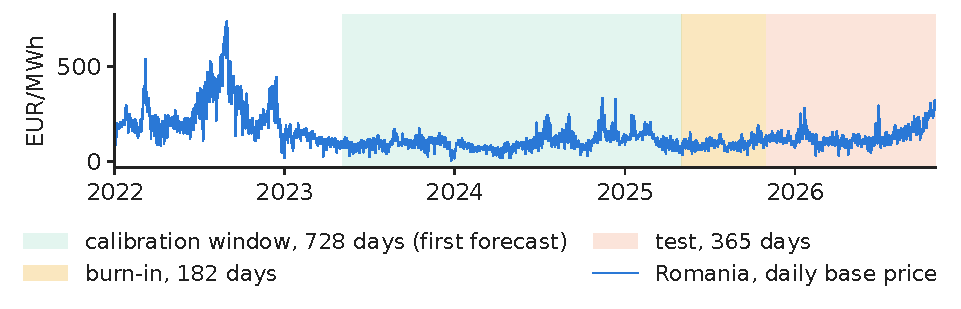
\includegraphics[width=\textwidth,height=0.520\textheight,keepaspectratio]{charts/en/split_timeline.pdf}\end{center}\vspace{-3mm}
\chartsource{Source: energy-charts.info (Fraunhofer ISE); OPCOM day-ahead prices for Romania, via ENTSO-E. Data: daily base price, 2022-01-01 to 2026-10-31, CET delivery days.}
\vspace{0.5mm}
\begin{itemize}\setlength{\itemsep}{0pt}
  \item Models re-estimated every day on the window ending at $d-1$
    \begin{itemize}\setlength{\itemsep}{0pt}
      \item No random K-fold, no random validation split.
    \end{itemize}
\end{itemize}
\par\vfill\manager{ask any vendor for the rolling backtest, not an in-sample fit.}\par\vspace{0.5mm}
\par\vfill\noindent{\scriptsize\color{FooterGray}(Weron, 2014, IJF; Lago, Marcjasz, De Schutter \& Weron, 2021, APEN)}\hfill\tryit{notebook \S1}\par\vspace{0.5mm}
\end{frame}

\begin{frame}{Older information, larger error, except at the weekly lag}
\small
\begin{center}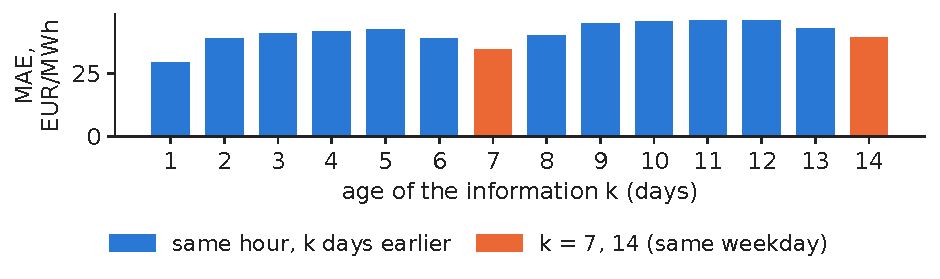
\includegraphics[width=\textwidth,height=0.452\textheight,keepaspectratio]{charts/en/horizon_naive.pdf}\end{center}\vspace{-3mm}
\chartsource{Source: energy-charts.info (Fraunhofer ISE); OPCOM day-ahead prices for Romania, via ENTSO-E. Data: test year 2025-11-01 to 2026-10-31, hourly.}
\vspace{0.5mm}
\begin{itemize}\setlength{\itemsep}{0pt}
  \item Forecast $\hat P_{d,h}=P_{d-k,h}$
    \begin{itemize}\setlength{\itemsep}{0pt}
      \item MAE 29.37 EUR/MWh for $k=1$, 38.52 for $k=2$, back to 34.41 for $k=7$ (same weekday).
    \end{itemize}
\end{itemize}
\par\vfill\manager{the day-ahead horizon is 12 to 36 hours
    \begin{itemize}\setlength{\itemsep}{0pt}
      \item The freshest price you hold at 12:00 is that of $d-1$.
    \end{itemize}}\par\vspace{0.5mm}
\par\vfill\noindent{\scriptsize\color{FooterGray}(own computation, test year 1 Nov 2025 -- 31 Oct 2026)}\hfill\tryit{notebook \S2}\par\vspace{0.5mm}
\end{frame}

\begin{frame}{Point, probabilistic and path forecasts answer different questions}
\footnotesize
\intuition{A point forecast gives one number per hour, a probabilistic one its distribution, a path forecast joint scenarios for the 24 hours.}
\begin{columns}[T,onlytextwidth]
\begin{column}{0.54\textwidth}
\[ \underbrace{\hat P_{d,h}}_{\text{point}}\quad\underbrace{\hat q^{\tau}_{d,h}:\ \Pr(P_{d,h}\le \hat q^{\tau}_{d,h})=\tau}_{\text{quantile}}\quad \underbrace{\{\hat P^{(s)}_{d,0},\dots,\hat P^{(s)}_{d,23}\}_{s=1}^{S}}_{\text{paths}} \]{\footnotesize\begin{itemize}\setlength{\itemsep}{0pt}
  \item \textbf{\txtwhere}
    \begin{itemize}\setlength{\itemsep}{0pt}
      \item $d$ = delivery day
      \item $h$ = hour (CET)
      \item $\tau\in(0,1)$ = quantile level
      \item $s$ = scenario
      \item $S$ = number of scenarios.
    \end{itemize}
\end{itemize}\par}
\end{column}
\begin{column}{0.43\textwidth}
\begin{itemize}\setlength{\itemsep}{1pt}
  \item \textbf{On our data}
    \begin{itemize}\setlength{\itemsep}{0pt}
      \item Errors at 12 h and 13 h correlate at 0.96
      \item Errors at 3 h and 19 h correlate at only 0.13
    \end{itemize}
  \item \textbf{Who needs what}
    \begin{itemize}\setlength{\itemsep}{0pt}
      \item Supplier buying a block, the point forecast
      \item Risk manager, quantiles (Lecture 4)
      \item Battery, paths, since it buys in one hour and sells in another
    \end{itemize}
\end{itemize}
\end{column}
\end{columns}
\par\vfill\manager{decide which of the three your decision needs before you buy a forecast.}\par\vspace{0.5mm}
\par\vfill\noindent{\scriptsize\color{FooterGray}(Nowotarski \& Weron, 2018, RSER)}\hfill\tryit{notebook \S7}\par\vspace{0.5mm}
\end{frame}

\subsection{Naive benchmarks and error measures}

\begin{frame}{The naive benchmark: yesterday, or last week for Monday and the weekend}
\footnotesize
\intuition{Every model must beat the rule a trader would use without any model.}
\begin{columns}[T,onlytextwidth]
\begin{column}{0.52\textwidth}
\[ \hat P^{\text{naive}}_{d,h}=\begin{cases}P_{d-7,h}, & \text{Mon, Sat, Sun}\\ P_{d-1,h}, & \text{Tue--Fri}\end{cases} \]\vspace{-2mm}\[ \hat P^{(7)}_{d,h}=P_{d-7,h} \]{\footnotesize\begin{itemize}\setlength{\itemsep}{0pt}
  \item \textbf{\txtwhere}
    \begin{itemize}\setlength{\itemsep}{0pt}
      \item $P_{d,h}$ = price of day $d$, hour $h$ (EUR/MWh)
      \item $\hat P^{(7)}$ = seasonal naive (same hour last week).
    \end{itemize}
\end{itemize}\par}
\end{column}
\begin{column}{0.45\textwidth}
\begin{itemize}\setlength{\itemsep}{1pt}
  \item \textbf{Why the switch}, MAE in EUR/MWh
    \begin{itemize}\setlength{\itemsep}{0pt}
      \item Mon, Sat, Sun: $d-7$ 29.87 vs $d-1$ 33.48
      \item Tue--Fri: $d-1$ 26.27 vs $d-7$ 37.83
    \end{itemize}
  \item \textbf{Test year}
    \begin{itemize}\setlength{\itemsep}{0pt}
      \item Naive 27.82, seasonal naive 34.41 EUR/MWh
      \item Mean price 134.46 EUR/MWh, so the naive error is about one fifth of the price
    \end{itemize}
\end{itemize}
\end{column}
\end{columns}
\par\vfill\manager{ask any forecast vendor for the rMAE against this naive rule on your hours.}\par\vspace{0.5mm}
\par\vfill\noindent{\scriptsize\color{FooterGray}(Nogales et al., 2002, IEEE TPWRS; Weron, 2014, IJF)}\hfill\tryit{notebook \S2}\par\vspace{0.5mm}
\end{frame}

\begin{frame}{Four error measures, one benchmark-relative score}
\footnotesize
\intuition{Absolute errors are in EUR/MWh, squared errors punish spikes, rMAE compares with naive.}
\begin{columns}[T,onlytextwidth]
\begin{column}{0.49\textwidth}
\[ \text{MAE}=\tfrac1N\textstyle\sum|e_{d,h}|,\quad \text{RMSE}=\sqrt{\tfrac1N\textstyle\sum e_{d,h}^2} \]\[ \text{sMAPE}=\tfrac1N\textstyle\sum\frac{2|e_{d,h}|}{|P_{d,h}|+|\hat P_{d,h}|},\quad \text{rMAE}=\frac{\text{MAE}_{\text{model}}}{\text{MAE}_{\text{naive}}} \]{\footnotesize\begin{itemize}\setlength{\itemsep}{0pt}
  \item \textbf{\txtwhere}
    \begin{itemize}\setlength{\itemsep}{0pt}
      \item $e_{d,h}=P_{d,h}-\hat P_{d,h}$
      \item $N$ = number of (day, hour) pairs
      \item Symmetric mean absolute percentage error (sMAPE), bounded by 200\%
      \item A value of rMAE below 1 = better than naive.
    \end{itemize}
\end{itemize}\par}
\end{column}
\begin{column}{0.48\textwidth}
\begin{itemize}\setlength{\itemsep}{1pt}
  \item \textbf{On our data}, test year 1 Nov 2025 -- 31 Oct 2026
    \begin{itemize}\setlength{\itemsep}{0pt}
      \item Naive: MAE 27.82, RMSE 44.54, sMAPE 34.5\%
      \item LEAR averaged across calibration windows (AW-LEAR): MAE 22.53, RMSE 36.35, rMAE 0.810
      \item Best, ensemble of 4: rMAE 0.795, i.e.\ 20.5\% less error than naive
    \end{itemize}
  \item MAE rewards the median forecast, RMSE the mean.
\end{itemize}
\end{column}
\end{columns}
\par\vfill\manager{report MAE in EUR/MWh to the desk and rMAE to management, on the same hours.}\par\vspace{0.5mm}
\par\vfill\noindent{\scriptsize\color{FooterGray}(Hyndman \& Koehler, 2006, IJF; Lago et al., 2021, APEN)}\hfill\tryit{notebook \S2}\par\vspace{0.5mm}
\end{frame}

\begin{frame}{Why percentage errors fail near zero and negative prices}
\small
\begin{center}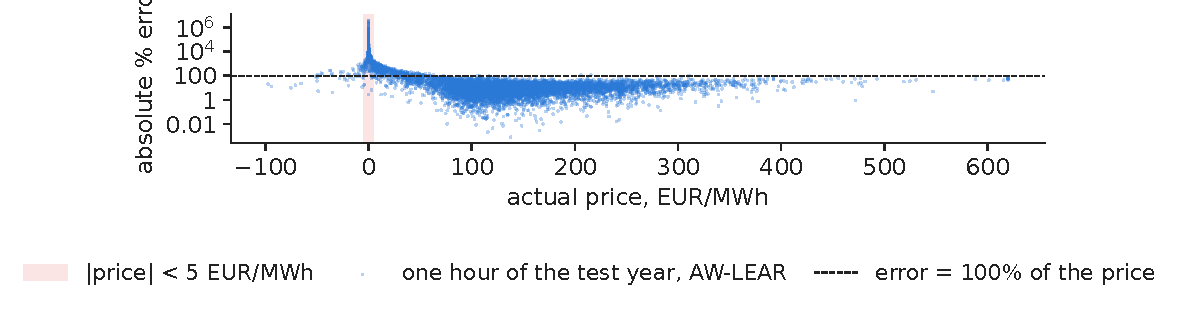
\includegraphics[width=\textwidth,height=0.407\textheight,keepaspectratio]{charts/en/mape_fail.pdf}\end{center}\vspace{-3mm}
\chartsource{Source: energy-charts.info (Fraunhofer ISE); OPCOM prices; ENTSO-E load, wind and solar (Transelectrica data for Romania). Data: test year 2025-11-01 to 2026-10-31, 8760 hours.}
\vspace{0.5mm}
\begin{itemize}\setlength{\itemsep}{0pt}
  \item Mean absolute percentage error (MAPE) $=\tfrac1N\sum|e_{d,h}|/|P_{d,h}|$
    \begin{itemize}\setlength{\itemsep}{0pt}
      \item For AW-LEAR 5\,777.7\%, or 32.4\% without the 387 hours with $|P|<5$ EUR/MWh.
    \end{itemize}
  \item These few hours produce 99.5\% of the MAPE.
\end{itemize}
\par\vfill\manager{never accept a MAPE for power prices
    \begin{itemize}\setlength{\itemsep}{0pt}
      \item Ask for MAE and rMAE.
    \end{itemize}}\par\vspace{0.5mm}
\par\vfill\noindent{\scriptsize\color{FooterGray}(Hyndman \& Koehler, 2006, IJF; Weron, 2014, IJF)}\hfill\tryit{notebook \S2}\par\vspace{0.5mm}
\end{frame}

\subsection{Testing forecast accuracy}

\begin{frame}{The Diebold--Mariano test: is the gain larger than luck?}
\footnotesize
\intuition{Compare the daily average error of two models; if the mean difference is large relative to its own noise, one model is really better.}
\begin{columns}[T,onlytextwidth]
\begin{column}{0.51\textwidth}
\[ \Delta_d=\underbrace{\tfrac1{24}\textstyle\sum_h|e^{A}_{d,h}|}_{\text{model A}}-\underbrace{\tfrac1{24}\textstyle\sum_h|e^{B}_{d,h}|}_{\text{model B}},\qquad \text{DM}=\frac{\bar\Delta}{\sqrt{\hat\sigma^2_{\Delta}/n}} \]{\footnotesize\begin{itemize}\setlength{\itemsep}{0pt}
  \item \textbf{\txtwhere}
    \begin{itemize}\setlength{\itemsep}{0pt}
      \item $n$ = test days
      \item $\hat\sigma^2_{\Delta}$ = Newey--West variance with 7 lags
      \item $p=1-\Phi(\text{DM})$
      \item Small $p$ = B more accurate than A.
    \end{itemize}
\end{itemize}\par}
\end{column}
\begin{column}{0.46\textwidth}
\begin{itemize}\setlength{\itemsep}{1pt}
  \item \textbf{On our data}, 365 test days
    \begin{itemize}\setlength{\itemsep}{0pt}
      \item Naive vs AW-LEAR: DM 7.32, $p$ $<$0.001
      \item ARX averaged across windows (AW-ARX) vs AW-LEAR: DM \ensuremath{-}0.83, $p$ = 0.797, no significant difference
      \item AW-LEAR vs ensemble of 4: DM 2.21, $p$ = 0.014
    \end{itemize}
  \item Daily averaging removes the correlation between the 24 hours of a day (multivariate version).
\end{itemize}
\end{column}
\end{columns}
\par\vfill\manager{switch models only when the gain is significant on your hours.}\par\vspace{0.5mm}
\par\vfill\noindent{\scriptsize\color{FooterGray}(Diebold \& Mariano, 1995, JBES; Ziel \& Weron, 2018, ENEECO)}\hfill\tryit{notebook \S2}\par\vspace{0.5mm}
\end{frame}

\begin{frame}{The DM chessboard: which model beats which on the Romanian test year}
\small
\begin{center}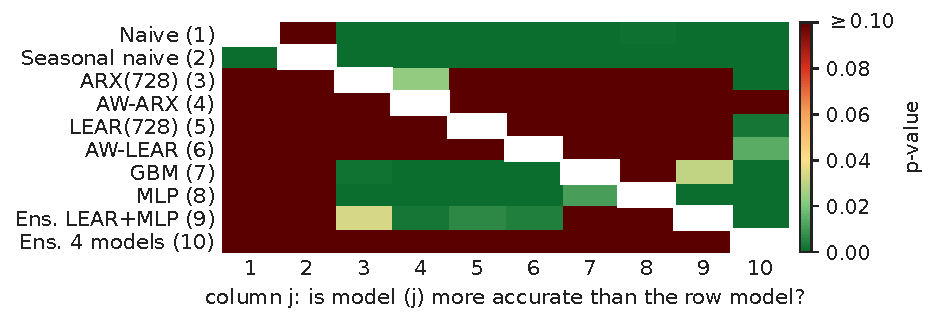
\includegraphics[width=\textwidth,height=0.473\textheight,keepaspectratio]{charts/en/dm_matrix.pdf}\end{center}\vspace{-3mm}
\chartsource{Source: energy-charts.info (Fraunhofer ISE); OPCOM prices; ENTSO-E generation and flows (Transelectrica data for Romania); Yahoo Finance (SparkChange EUA ETC). Data: test year 2025-11-01 to 2026-10-31, 365 days; one-sided p-values.}
\vspace{0.5mm}
\begin{itemize}\setlength{\itemsep}{0pt}
  \item 8 of the 9 other models beat the naive benchmark at 5\%
    \begin{itemize}\setlength{\itemsep}{0pt}
      \item Green cells mark a significant win of the column.
    \end{itemize}
\end{itemize}
\par\vfill\manager{read a column top to bottom
    \begin{itemize}\setlength{\itemsep}{0pt}
      \item Many green cells mean a model worth paying for.
    \end{itemize}}\par\vspace{0.5mm}
\par\vfill\noindent{\scriptsize\color{FooterGray}(Ziel \& Weron, 2018, ENEECO; Lago et al., 2021, APEN)}\hfill\tryit{notebook \S2}\par\vspace{0.5mm}
\end{frame}


\section{Expert models: ARX and LEAR}

\subsection{The expert ARX model}

\begin{frame}{The expert ARX model: recent prices, calendar and fundamentals}
\footnotesize
\intuition{One linear regression per hour, with the inputs a trader looks at first.}
\begin{columns}[T,onlytextwidth]
\begin{column}{0.55\textwidth}
\[ \begin{aligned} Y_{d,h}=\beta_0&+\underbrace{\beta_1Y_{d-1,h}+\beta_2Y_{d-2,h}+\beta_3Y_{d-7,h}}_{\text{autoregression}}\\&+\underbrace{\beta_4Y_{d-1,23}+\beta_5Y^{\min}_{d-1}+\beta_6Y^{\max}_{d-1}}_{\text{yesterday's shape}}\\&+\underbrace{\beta_7\tilde L_{d,h}+\beta_8\tilde R_{d,h}}_{\text{fundamentals of } d-2}+\underbrace{\textstyle\sum_{j}\delta_jD^{j}_d}_{\text{Mon, Sat, Sun}}+\varepsilon_{d,h} \end{aligned} \]{\footnotesize\begin{itemize}\setlength{\itemsep}{0pt}
  \item \textbf{\txtwhere}
    \begin{itemize}\setlength{\itemsep}{0pt}
      \item $Y$ = asinh-transformed price
      \item $\tilde L_{d,h}=L_{d-2,h}$ load, $\tilde R_{d,h}$ wind + solar of $d-2$, z-scored.
    \end{itemize}
\end{itemize}\par}
\end{column}
\begin{column}{0.42\textwidth}
\begin{itemize}\setlength{\itemsep}{1pt}
  \item \textbf{Estimation}
    \begin{itemize}\setlength{\itemsep}{0pt}
      \item Ordinary least squares (OLS), separately for each $h$
      \item 12 regressors per hour, as in Assignment 1
    \end{itemize}
  \item \textbf{On our data}, ARX(728)
    \begin{itemize}\setlength{\itemsep}{0pt}
      \item 728-day window, re-estimated daily
      \item MAE 22.72 EUR/MWh, rMAE 0.817
    \end{itemize}
\end{itemize}
\end{column}
\end{columns}
\par\vfill\manager{this is the model to beat before anyone sells you a neural network.}\par\vspace{0.5mm}
\par\vfill\noindent{\scriptsize\color{FooterGray}(Ziel \& Weron, 2018, ENEECO; Weron, 2014, IJF)}\hfill\tryit{notebook \S3}\par\vspace{0.5mm}
\end{frame}

\begin{frame}{The ARX coefficients change with the hour of the day}
\small
\begin{center}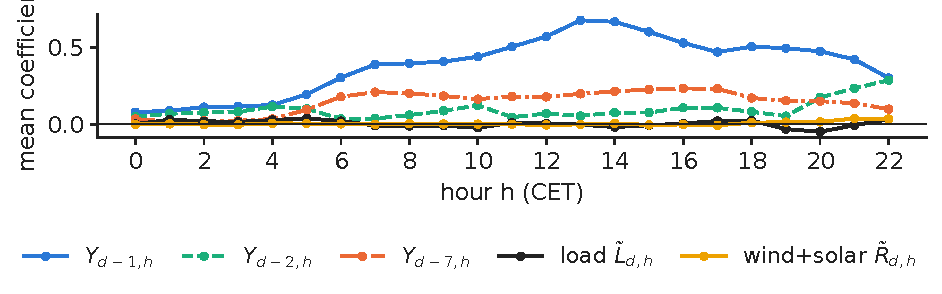
\includegraphics[width=\textwidth,height=0.467\textheight,keepaspectratio]{charts/en/arx_coef.pdf}\end{center}\vspace{-3mm}
\chartsource{Source: energy-charts.info (Fraunhofer ISE); OPCOM prices; ENTSO-E load, wind and solar (Transelectrica data for Romania). Data: ARX(728), mean over the 365 daily fits of the test year.}
\vspace{0.5mm}
\begin{itemize}\setlength{\itemsep}{0pt}
  \item $Y_{d-1,h}$ weighs most at hour 13 (0.68) and least at hour 0 (0.08)
    \begin{itemize}\setlength{\itemsep}{0pt}
      \item Night hours lean on the last hour of $d-1$ instead (up to 0.73).
    \end{itemize}
  \item The load and wind + solar coefficients stay close to zero: at $d-2$ they add little to yesterday's price.
\end{itemize}
\par\vfill\manager{one model per hour lets the evening peak learn from different drivers than the night.}\par\vspace{0.5mm}
\par\vfill\noindent{\scriptsize\color{FooterGray}(own estimation, ARX(728))}\hfill\tryit{notebook \S3}\par\vspace{0.5mm}
\end{frame}

\begin{frame}{Fundamentals lagged by two days add almost nothing}
\footnotesize
\begin{columns}[T,onlytextwidth]
\begin{column}{0.50\textwidth}
{\footnotesize\renewcommand{\arraystretch}{1.25}\setlength{\tabcolsep}{4pt}
\begin{tabular}{@{}p{0.52\linewidth}rrr@{}}\toprule
ARX(728), test year & MAE & RMSE & rMAE \\ \midrule
prices and calendar only & 22.63 & 36.49 & 0.813 \\
+ load, wind + solar of $d-2$ & 22.72 & 36.62 & 0.817 \\
+ hydro, nuclear, net imports, EUA of $d-2$ & 22.72 & 36.50 & 0.817 \\
\bottomrule\end{tabular}}
\par\vspace{0.5mm}{\scriptsize \begin{itemize}\setlength{\itemsep}{0pt}
  \item Fundamentals missing on a day are carried forward from the past only (nuclear on 29 days).
  \item EUA = SparkChange ETC close of $d-2$, a proxy of the allowance price.
\end{itemize}}
\end{column}
\begin{column}{0.47\textwidth}
\begin{itemize}\setlength{\itemsep}{1pt}
  \item \textbf{Why so little}
    \begin{itemize}\setlength{\itemsep}{0pt}
      \item What happened on $d-2$ is already in the price of $d-1$
      \item The outages of the Cernavodă nuclear power plant reach the model two days late
    \end{itemize}
  \item \textbf{What would help}
    \begin{itemize}\setlength{\itemsep}{0pt}
      \item Published day-ahead forecasts of load, wind and solar for day $d$ (ENTSO-E, Transelectrica)
      \item They are legal at 12:00 on $d-1$, but not in our free data
    \end{itemize}
\end{itemize}
\end{column}
\end{columns}
\par\vfill\manager{buy the TSO's day-ahead load and renewable forecasts before buying a more complex model.}\par\vspace{0.5mm}
\par\vfill\noindent{\scriptsize\color{FooterGray}(own estimation; Lago et al., 2021, APEN)}\hfill\tryit{notebook \S3}\par\vspace{0.5mm}
\end{frame}

\begin{frame}{One model per hour beats one model for all hours}
\small
\begin{center}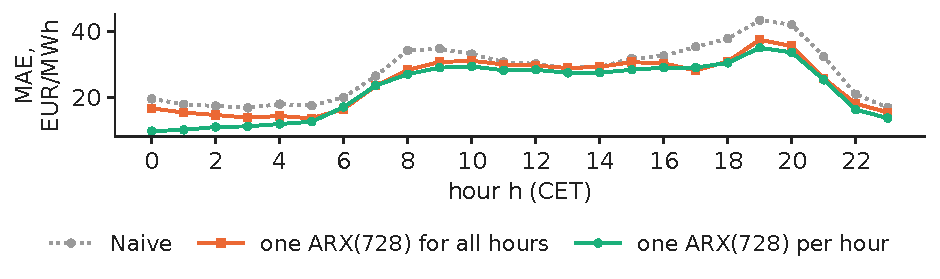
\includegraphics[width=\textwidth,height=0.500\textheight,keepaspectratio]{charts/en/per_hour_single.pdf}\end{center}\vspace{-3mm}
\chartsource{Source: energy-charts.info (Fraunhofer ISE); OPCOM prices; ENTSO-E load, wind and solar (Transelectrica data for Romania). Data: test year 2025-11-01 to 2026-10-31.}
\vspace{0.5mm}
\begin{itemize}\setlength{\itemsep}{0pt}
  \item MAE 22.72 per hour vs 24.54 EUR/MWh pooled (hour intercepts, common slopes)
    \begin{itemize}\setlength{\itemsep}{0pt}
      \item Pooled worse in 21 of 24 hours.
    \end{itemize}
\end{itemize}
\par\vfill\manager{since 1 Oct 2025 the same choice arises for the 96 quarter-hours.}\par\vspace{0.5mm}
\par\vfill\noindent{\scriptsize\color{FooterGray}(Ziel \& Weron, 2018, ENEECO)}\hfill\tryit{notebook \S3}\par\vspace{0.5mm}
\end{frame}

\subsection{Variance-stabilising transformations}

\begin{frame}{The asinh transformation tames spikes and negative prices}
\small
\begin{center}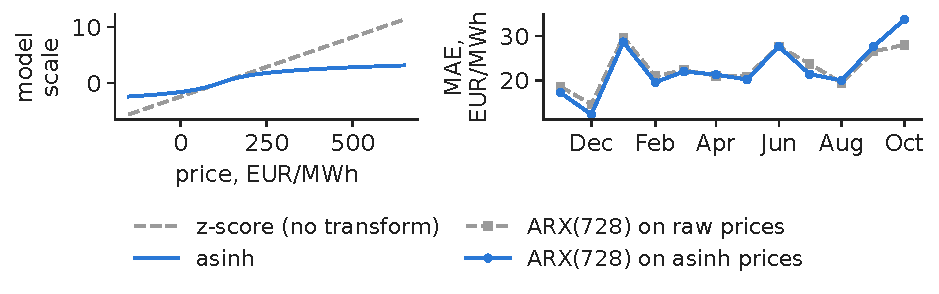
\includegraphics[width=\textwidth,height=0.424\textheight,keepaspectratio]{charts/en/vst.pdf}\end{center}\vspace{-3mm}
\chartsource{Source: energy-charts.info (Fraunhofer ISE); OPCOM prices; ENTSO-E load, wind and solar (Transelectrica data for Romania). Data: left, median and scale of the last window; right, test year 2025-11-01 to 2026-10-31.}
\vspace{0.5mm}
\begin{itemize}\setlength{\itemsep}{0pt}
  \item Variance-stabilising transformation (VST) $Y=\asinh((P-m)/s)$, $m$ = median, $s$ = 1.4826 $\times$ median absolute deviation (MAD), from the window only.
  \item ARX(728) MAE 22.86 raw vs 22.72 with asinh
    \begin{itemize}\setlength{\itemsep}{0pt}
      \item RMSE goes the other way (35.85 vs 36.62).
    \end{itemize}
\end{itemize}
\par\vfill\manager{asinh works below zero, where the logarithm cannot be used.}\par\vspace{0.5mm}
\par\vfill\noindent{\scriptsize\color{FooterGray}(Uniejewski, Weron \& Ziel, 2018, IEEE TPWRS)}\hfill\tryit{notebook \S3}\par\vspace{0.5mm}
\end{frame}

\subsection{LASSO-estimated autoregression}

\begin{frame}{LEAR: give the model 247 candidates and let the LASSO switch most of them off}
\footnotesize
\intuition{A penalty on the size of the coefficients sets the useless ones exactly to zero, so the data choose the regressors.}
\begin{columns}[T,onlytextwidth]
\begin{column}{0.53\textwidth}
\[ \hat{\bm\beta}_h=\arg\min_{\bm\beta}\Big\{\underbrace{\textstyle\sum_{d\in\text{cal}}(Y_{d,h}-\mathbf x_d^{\top}\bm\beta)^2}_{\text{fit}}+\underbrace{\lambda_h\textstyle\sum_j|\beta_j|}_{\text{penalty}}\Big\} \]{\footnotesize\begin{itemize}\setlength{\itemsep}{0pt}
  \item \textbf{\txtwhere}
    \begin{itemize}\setlength{\itemsep}{0pt}
      \item $\mathbf x_d$ = 247 regressors, all 24 prices of $d-1,d-2,d-3,d-7$ (96), load and wind + solar of $d-2,d-3,d-7$ (144), 7 weekday dummies
      \item $\lambda_h$ chosen every day by the Akaike information criterion (AIC) inside the window.
    \end{itemize}
\end{itemize}\par}
\end{column}
\begin{column}{0.44\textwidth}
\begin{itemize}\setlength{\itemsep}{1pt}
  \item \textbf{On our data}, LEAR(728)
    \begin{itemize}\setlength{\itemsep}{0pt}
      \item On average 42 of 247 regressors kept (17\%), from 8 to 121
      \item MAE 22.62; averaged over 364, 546, 728 days (AW-LEAR) 22.53 EUR/MWh
    \end{itemize}
  \item \textbf{Choosing $\lambda$ honestly}
    \begin{itemize}\setlength{\itemsep}{0pt}
      \item By an information criterion, or on a validation block that ends before the forecast day
      \item Never on the test year
    \end{itemize}
\end{itemize}
\end{column}
\end{columns}
\par\vfill\manager{a LASSO model explains itself, since the kept regressors show what drives each hour.}\par\vspace{0.5mm}
\par\vfill\noindent{\scriptsize\color{FooterGray}(Tibshirani, 1996; Uniejewski, Nowotarski \& Weron, 2016; Lago et al., 2021)}\hfill\tryit{notebook \S4}\par\vspace{0.5mm}
\end{frame}

\begin{frame}{What LEAR keeps: yesterday's same hour and the weekday, rarely the lagged fundamentals}
\small
\begin{center}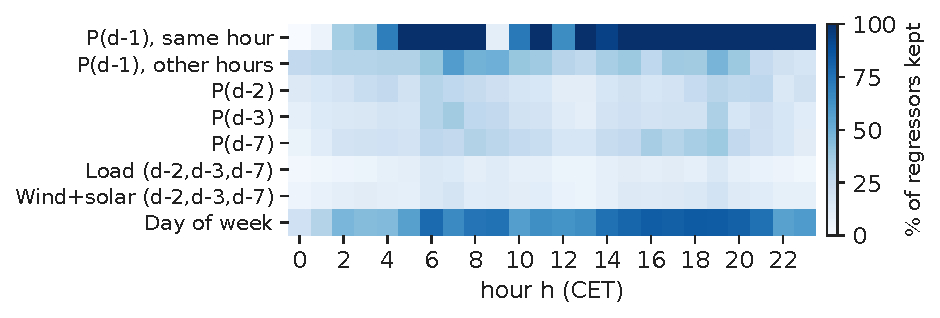
\includegraphics[width=\textwidth,height=0.492\textheight,keepaspectratio]{charts/en/lear_sel.pdf}\end{center}\vspace{-3mm}
\chartsource{Source: energy-charts.info (Fraunhofer ISE); OPCOM prices; ENTSO-E load, wind and solar (Transelectrica data for Romania). Data: LEAR(728), 365 daily fits of the test year.}
\vspace{0.5mm}
\begin{itemize}\setlength{\itemsep}{0pt}
  \item Kept on average, $P_{d-1,h}$ 79\%, weekday 64\%, load 9\%, wind + solar 11\% of the regressors.
\end{itemize}
\par\vfill\manager{real gains need forecasts of the fundamentals for day $d$.}\par\vspace{0.5mm}
\par\vfill\noindent{\scriptsize\color{FooterGray}(own estimation, LEAR(728), test year 1 Nov 2025 -- 31 Oct 2026)}\hfill\tryit{notebook \S4}\par\vspace{0.5mm}
\end{frame}


\section{Windows, combinations and machine learning}

\subsection{Calibration windows}

\begin{frame}{Short windows adapt, long windows are stable: average them}
\footnotesize
\intuition{Instead of guessing the best window length, estimate the model on several windows and average the forecasts.}
\begin{columns}[T,onlytextwidth]
\begin{column}{0.52\textwidth}
\[ \hat P^{\text{AW}}_{d,h}=\frac1{|\mathcal T|}\sum_{T\in\mathcal T}\underbrace{\hat P^{(T)}_{d,h}}_{\text{window of } T \text{ days}} \]{\footnotesize\begin{itemize}\setlength{\itemsep}{0pt}
  \item \textbf{\txtwhere}
    \begin{itemize}\setlength{\itemsep}{0pt}
      \item Rolling window = last $T$ days, re-estimated daily
      \item ARX: $\mathcal T=\{56,84,112,714,721,728\}$
      \item LEAR: $\mathcal T=\{364,546,728\}$
      \item Averaging across calibration windows (AW).
    \end{itemize}
\end{itemize}\par}
\end{column}
\begin{column}{0.45\textwidth}
\begin{itemize}\setlength{\itemsep}{1pt}
  \item \textbf{On our data}, MAE in EUR/MWh
    \begin{itemize}\setlength{\itemsep}{0pt}
      \item ARX(56) 24.44, ARX(112) 23.41, ARX(728) 22.72
      \item AW-ARX 22.30, better than every single window
      \item LEAR(364) 22.96, LEAR(728) 22.62, AW-LEAR 22.53
    \end{itemize}
  \item Mixing short (56--112) and long (714--728) windows gives both adaptation and stability.
\end{itemize}
\end{column}
\end{columns}
\par\vfill\manager{when the market changes regime (2022, 2024), short windows react first
    \begin{itemize}\setlength{\itemsep}{0pt}
      \item Keep them in the average.
    \end{itemize}}\par\vspace{0.5mm}
\par\vfill\noindent{\scriptsize\color{FooterGray}(Hubicka, Marcjasz \& Weron, 2019; Marcjasz, Serafin \& Weron, 2018)}\hfill\tryit{notebook \S5}\par\vspace{0.5mm}
\end{frame}

\begin{frame}{Averaging across windows beats the best single window}
\small
\begin{center}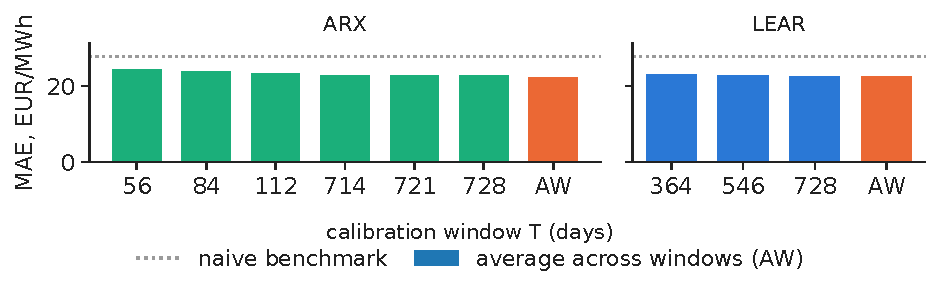
\includegraphics[width=\textwidth,height=0.466\textheight,keepaspectratio]{charts/en/windows.pdf}\end{center}\vspace{-3mm}
\chartsource{Source: energy-charts.info (Fraunhofer ISE); OPCOM prices; ENTSO-E load, wind and solar (Transelectrica data for Romania). Data: test year 2025-11-01 to 2026-10-31.}
\vspace{0.5mm}
\begin{itemize}\setlength{\itemsep}{0pt}
  \item AW-ARX 22.30 vs the best single window ARX(714) 22.68
    \begin{itemize}\setlength{\itemsep}{0pt}
      \item Dotted line = naive 27.82 EUR/MWh.
    \end{itemize}
\end{itemize}
\par\vfill\manager{you do not need to know the right window in advance
    \begin{itemize}\setlength{\itemsep}{0pt}
      \item Average a short and a long one.
    \end{itemize}}\par\vspace{0.5mm}
\par\vfill\noindent{\scriptsize\color{FooterGray}(Hubicka, Marcjasz \& Weron, 2019, IEEE TSTE)}\hfill\tryit{notebook \S5}\par\vspace{0.5mm}
\end{frame}

\subsection{Combining forecasts}

\begin{frame}{Combining different models: errors that do not coincide cancel out}
\footnotesize
\intuition{If two models are wrong on different days, their simple average is wrong less often than either.}
\begin{columns}[T,onlytextwidth]
\begin{column}{0.48\textwidth}
\[ \hat P^{\text{ens}}_{d,h}=\frac1K\sum_{k=1}^{K}\hat P^{(k)}_{d,h},\quad \Var(\bar e)=\frac{\bar\sigma^2}{K}\big(1+(K-1)\bar\rho\big) \]{\footnotesize\begin{itemize}\setlength{\itemsep}{0pt}
  \item \textbf{\txtwhere}
    \begin{itemize}\setlength{\itemsep}{0pt}
      \item $K$ = number of models
      \item $\bar\sigma^2$ = average error variance
      \item $\bar\rho$ = average correlation of the errors
      \item The lower $\bar\rho$, the larger the gain
      \item Equal weights need no estimation.
    \end{itemize}
\end{itemize}\par}
\end{column}
\begin{column}{0.49\textwidth}
\begin{itemize}\setlength{\itemsep}{1pt}
  \item \textbf{On our data}, ensemble of 4
    \begin{itemize}\setlength{\itemsep}{0pt}
      \item AW-ARX, AW-LEAR, a gradient boosting machine (GBM) and a multilayer perceptron (MLP), equal weights
      \item MAE 22.13 EUR/MWh, rMAE 0.795, the best of all models
      \item Better than AW-LEAR in 8 of 12 months and in 15 of 24 hours
      \item DM test against AW-LEAR: $p$ = 0.014
    \end{itemize}
  \item The two weaker members (GBM, MLP) still help, because their errors differ.
\end{itemize}
\end{column}
\end{columns}
\par\vfill\manager{ask vendors for forecasts you can average with yours, not for a single best model.}\par\vspace{0.5mm}
\par\vfill\noindent{\scriptsize\color{FooterGray}(Bates \& Granger, 1969; Nowotarski \& Weron, 2015)}\hfill\tryit{notebook \S5}\par\vspace{0.5mm}
\end{frame}

\begin{frame}{Results on the Romanian test year: the scoreboard}
\small
\begin{center}{\scriptsize\renewcommand{\arraystretch}{1.02}\setlength{\tabcolsep}{4pt}
\begin{tabular}{@{}lrrrr@{}}\toprule
Model & MAE & RMSE & sMAPE, \% & rMAE \\ \midrule
Naive & \cellcolor{Forest!4}27.82 & \cellcolor{Forest!6}44.54 & \cellcolor{Crimson!10}34.5 & \cellcolor{Forest!4}1.000 \\
Seasonal naive & \cellcolor{Crimson!55}34.41 & \cellcolor{Crimson!55}55.48 & \cellcolor{Crimson!55}39.4 & \cellcolor{Crimson!55}1.237 \\
ARX(56) & \cellcolor{Forest!34}24.44 & \cellcolor{Forest!31}40.09 & \cellcolor{Forest!31}30.0 & \cellcolor{Forest!34}0.879 \\
ARX(728) & \cellcolor{Forest!50}22.72 & \cellcolor{Forest!50}36.62 & \cellcolor{Forest!51}27.8 & \cellcolor{Forest!50}0.817 \\
AW-ARX & \cellcolor{Forest!53}22.30 & \cellcolor{Forest!52}36.34 & \cellcolor{Forest!54}27.6 & \cellcolor{Forest!53}0.802 \\
ARX(728), one model & \cellcolor{Forest!33}24.54 & \cellcolor{Forest!43}37.97 & \cellcolor{Forest!36}29.5 & \cellcolor{Forest!33}0.882 \\
ARX(728), no VST & \cellcolor{Forest!48}22.86 & \cellcolor{Forest!54}35.85 & \cellcolor{Forest!46}28.4 & \cellcolor{Forest!48}0.822 \\
LEAR(364) & \cellcolor{Forest!48}22.96 & \cellcolor{Forest!49}36.80 & \cellcolor{Forest!49}28.1 & \cellcolor{Forest!48}0.825 \\
LEAR(728) & \cellcolor{Forest!51}22.62 & \cellcolor{Forest!52}36.36 & \cellcolor{Forest!53}27.7 & \cellcolor{Forest!51}0.813 \\
AW-LEAR & \cellcolor{Forest!51}22.53 & \cellcolor{Forest!52}36.35 & \cellcolor{Forest!53}27.7 & \cellcolor{Forest!51}0.810 \\
GBM & \cellcolor{Forest!38}24.05 & \cellcolor{Forest!44}37.73 & \cellcolor{Forest!44}28.7 & \cellcolor{Forest!38}0.864 \\
MLP & \cellcolor{Forest!24}25.54 & \cellcolor{Forest!31}40.05 & \cellcolor{Forest!33}29.8 & \cellcolor{Forest!24}0.918 \\
Ensemble LEAR+MLP & \cellcolor{Forest!46}23.12 & \cellcolor{Forest!48}36.95 & \cellcolor{Forest!49}28.1 & \cellcolor{Forest!46}0.831 \\
Ensemble of 4 & \cellcolor{Forest!55}22.13 & \cellcolor{Forest!55}35.76 & \cellcolor{Forest!55}27.4 & \cellcolor{Forest!55}0.795 \\
\bottomrule\end{tabular}}\end{center}\vspace{-2mm}
\par\vspace{0.5mm}{\scriptsize \begin{itemize}\setlength{\itemsep}{0pt}
  \item Test year 1 Nov 2025 -- 31 Oct 2026, 8\,760 hours; green = better, red = worse, per column.
  \item Without the 2 DST days the MAE of AW-LEAR is 22.48; the ranking does not change.
\end{itemize}}
\par\vfill\noindent{\scriptsize\color{FooterGray}(Weron, 2014, IJF; Lago, Marcjasz, De Schutter \& Weron, 2021, APEN)}\hfill\tryit{notebook \S5}\par\vspace{0.5mm}
\end{frame}

\subsection{Machine learning: a preview of Lecture 7}

\begin{frame}{Gradient boosting: many small trees, each correcting the previous ones}
\footnotesize
\intuition{Trees capture thresholds and interactions (e.g.\ low wind and high load in the evening) that a linear model misses.}
\begin{columns}[T,onlytextwidth]
\begin{column}{0.50\textwidth}
\[ F_m(\mathbf x)=F_{m-1}(\mathbf x)+\nu\,f_m(\mathbf x) \]\vspace{-2mm}\[ f_m=\arg\min_f\textstyle\sum_i\big(r_i^{(m)}-f(\mathbf x_i)\big)^2 \]{\footnotesize\begin{itemize}\setlength{\itemsep}{0pt}
  \item \textbf{\txtwhere}
    \begin{itemize}\setlength{\itemsep}{0pt}
      \item $f_m$ = small regression tree
      \item $r_i^{(m)}=Y_i-F_{m-1}(\mathbf x_i)$ = current residual
      \item $\nu=0.05$ = learning rate
      \item 500 trees fixed in advance.
    \end{itemize}
\end{itemize}\par}
\end{column}
\begin{column}{0.47\textwidth}
\begin{itemize}\setlength{\itemsep}{1pt}
  \item \textbf{Our gradient boosting machine (GBM)}
    \begin{itemize}\setlength{\itemsep}{0pt}
      \item One model for all hours, with the hour as a feature; 20 features, all available at 12:00 on $d-1$
      \item Refitted at the start of each of the 12 test months on all days before it (expanding window)
    \end{itemize}
  \item \textbf{Result}
    \begin{itemize}\setlength{\itemsep}{0pt}
      \item MAE 24.05, rMAE 0.864; behind AW-LEAR over the year
      \item But the best single model in the stress week (MAE 34.35)
    \end{itemize}
\end{itemize}
\end{column}
\end{columns}
\par\vfill\manager{trees are worth adding to an ensemble even when they do not win alone.}\par\vspace{0.5mm}
\par\vfill\noindent{\scriptsize\color{FooterGray}(Friedman, 2001, Ann.\ Stat.; Lago et al., 2021, APEN)}\hfill\tryit{notebook \S6}\par\vspace{0.5mm}
\end{frame}

\begin{frame}{Neural networks: 24 prices out of one input vector}
\footnotesize
\intuition{A multi-output network forecasts the whole day at once, like the deep neural network (DNN) of Lago et al.}
\begin{columns}[T,onlytextwidth]
\begin{column}{0.50\textwidth}
\[ \hat{\mathbf Y}_d=W_3\,\phi\big(W_2\,\phi(W_1\mathbf x_d+b_1)+b_2\big)+b_3\in\mathbb R^{24} \]{\footnotesize\begin{itemize}\setlength{\itemsep}{0pt}
  \item \textbf{\txtwhere}
    \begin{itemize}\setlength{\itemsep}{0pt}
      \item $\mathbf x_d$ = the 247 LEAR regressors + 4 fundamentals of $d-2$
      \item $\phi$ = rectified linear unit (ReLU)
      \item Layers of 128 and 64 neurons
      \item Multilayer perceptron (MLP).
    \end{itemize}
\end{itemize}\par}
\end{column}
\begin{column}{0.47\textwidth}
\begin{itemize}\setlength{\itemsep}{1pt}
  \item \textbf{Time-series discipline}
    \begin{itemize}\setlength{\itemsep}{0pt}
      \item Epochs chosen on the last 15\% of the training days, in time order (median 20)
      \item 4 seeds averaged; refitted monthly, scaling fitted on training days only
    \end{itemize}
  \item \textbf{Result}
    \begin{itemize}\setlength{\itemsep}{0pt}
      \item MAE 25.54, rMAE 0.918; a small untuned network does not beat LEAR
      \item The tuned DNN of Lago et al.\ (2021) does better (Lecture 7)
    \end{itemize}
\end{itemize}
\end{column}
\end{columns}
\par\vfill\manager{a neural network needs years of data and careful tuning, or you keep LEAR.}\par\vspace{0.5mm}
\par\vfill\noindent{\scriptsize\color{FooterGray}(Lago, Marcjasz, De Schutter \& Weron, 2021, APEN)}\hfill\tryit{notebook \S6}\par\vspace{0.5mm}
\end{frame}

\begin{frame}{Hour by hour: machine learning helps inside the ensemble, not alone}
\small
\begin{center}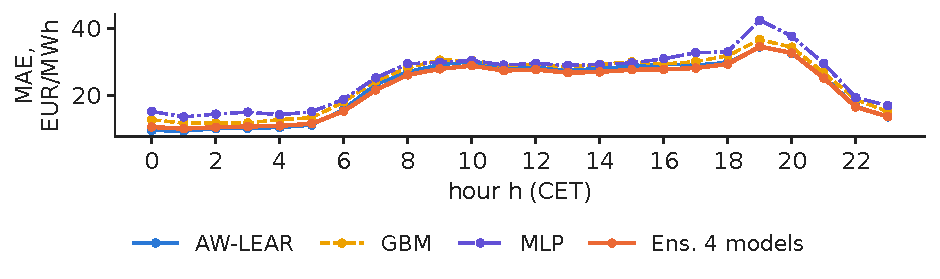
\includegraphics[width=\textwidth,height=0.500\textheight,keepaspectratio]{charts/en/ml_hour.pdf}\end{center}\vspace{-3mm}
\chartsource{Source: energy-charts.info (Fraunhofer ISE); OPCOM prices; ENTSO-E generation and flows (Transelectrica data for Romania); Yahoo Finance (SparkChange EUA ETC). Data: test year 2025-11-01 to 2026-10-31; ML refitted monthly.}
\vspace{0.5mm}
\begin{itemize}\setlength{\itemsep}{0pt}
  \item Better than AW-LEAR in 0 hours (GBM), 0 (MLP) and 15 of 24 (ensemble of 4).
  \item The hardest hour is 19 h CET, the evening ramp (AW-LEAR MAE 34.52 EUR/MWh).
\end{itemize}
\par\vfill\manager{put your best analyst on the evening hours, where the money is lost.}\par\vspace{0.5mm}
\par\vfill\noindent{\scriptsize\color{FooterGray}(own computation, test year 1 Nov 2025 -- 31 Oct 2026)}\hfill\tryit{notebook \S6}\par\vspace{0.5mm}
\end{frame}

\begin{frame}{Our group on Romanian load: machine learning wins when the series is smooth}
\footnotesize
\begin{itemize}\setlength{\itemsep}{1pt}
  \item \textbf{The study} (Proșcanu, Proșcanu, Pele \& Costea, 2025)
    \begin{itemize}\setlength{\itemsep}{0pt}
      \item Hourly national load of Romania, 2022--2024; classical seasonal models against neural networks
    \end{itemize}
  \item \textbf{Our replication} (studiu de caz C2, same gate-closure rule)
    \begin{itemize}\setlength{\itemsep}{0pt}
      \item 217 test days from 27 May 2024; load metered up to $d-2$
      \item MAPE: gradient boosting 4.09\%, Chronos-Bolt foundation model 4.16\%, MLP 4.58\%
      \item Linear regression 4.85\%, seasonal autoregressive model 8.03\%, naive two days earlier 10.17\%
    \end{itemize}
  \item \textbf{Why the contrast with prices}
    \begin{itemize}\setlength{\itemsep}{0pt}
      \item Load is smooth and never near zero, so MAPE is meaningful and nonlinear models have patterns to learn
      \item Prices jump and turn negative; there, a well-built linear model is hard to beat
    \end{itemize}
\end{itemize}
\par\vspace{0.5mm}{\scriptsize \begin{itemize}\setlength{\itemsep}{0pt}
  \item C2 figures are computed by the C2 case notebook on our data; the paper's own results are in the case brief.
\end{itemize}}
\par\vfill\manager{forecast your own load with ML and the price with LEAR plus an ensemble.}\par\vspace{0.5mm}
\par\vfill\noindent{\scriptsize\color{FooterGray}(Proșcanu, Proșcanu, Pele \& Costea, 2025, RJEF; case study C2)}\par\vspace{0.5mm}
\end{frame}


\section{Probabilistic forecasts and cointegration}

\subsection{Quantile regression averaging}

\begin{frame}{Quantile regression averaging: from point forecasts to quantiles}
\footnotesize
\intuition{Regress the actual price on several point forecasts, once per quantile level, and the forecasts become a distribution.}
\begin{columns}[T,onlytextwidth]
\begin{column}{0.52\textwidth}
\[ \hat q^{\tau}_{d,h}=\beta^{\tau}_{0,h}+\beta^{\tau}_{1,h}\hat P^{\text{AW-ARX}}_{d,h}+\beta^{\tau}_{2,h}\hat P^{\text{AW-LEAR}}_{d,h} \]\[ \text{PS}_\tau(q,y)=\big(\mathbb 1\{y<q\}-\tau\big)(q-y) \]{\footnotesize\begin{itemize}\setlength{\itemsep}{0pt}
  \item \textbf{\txtwhere}
    \begin{itemize}\setlength{\itemsep}{0pt}
      \item $\bm\beta^{\tau}_h$ minimises the pinball score (PS) on the last 182 days of forecasts, re-estimated weekly
      \item $\tau=0.01,\dots,0.99$.
    \end{itemize}
\end{itemize}\par}
\end{column}
\begin{column}{0.45\textwidth}
\begin{itemize}\setlength{\itemsep}{1pt}
  \item \textbf{On our data}, average pinball score
    \begin{itemize}\setlength{\itemsep}{0pt}
      \item QRA 8.33; conformal prediction (CP) 8.47; historical simulation (HS) 8.41
      \item CP and HS use the AW-LEAR errors of the last 112 days, as in Assignment 1
    \end{itemize}
  \item \textbf{Coverage of the 90\% interval}
    \begin{itemize}\setlength{\itemsep}{0pt}
      \item QRA 85.7\%, CP 87.0\%, HS 85.8\%; mean QRA width 93.0 EUR/MWh
      \item All below 90\%; the Kupiec test rejects correct coverage
    \end{itemize}
\end{itemize}
\end{column}
\end{columns}
\par\vfill\manager{a 90\% band that holds 86\% of the prices understates the risk of the open position.}\par\vspace{0.5mm}
\par\vfill\noindent{\scriptsize\color{FooterGray}(Koenker \& Bassett, 1978; Nowotarski \& Weron, 2015)}\hfill\tryit{notebook \S7}\par\vspace{0.5mm}
\end{frame}

\begin{frame}{A week of QRA intervals in Romania: wide in the evening, narrow at night}
\small
\begin{center}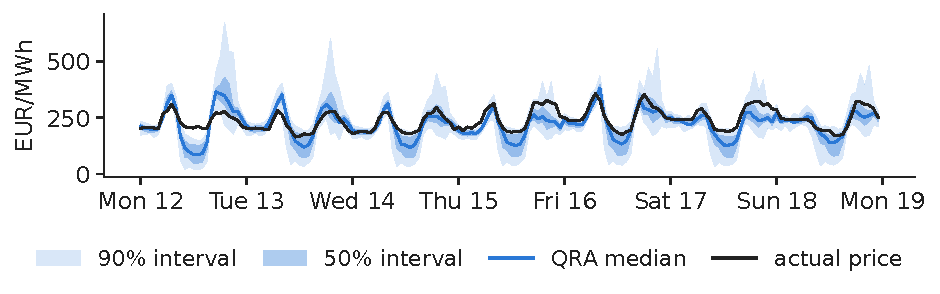
\includegraphics[width=\textwidth,height=0.461\textheight,keepaspectratio]{charts/en/qra_week.pdf}\end{center}\vspace{-3mm}
\chartsource{Source: energy-charts.info (Fraunhofer ISE); OPCOM prices; ENTSO-E load, wind and solar (Transelectrica data for Romania). Data: week 2026-10-12 to 2026-10-18, hourly.}
\vspace{0.5mm}
\begin{itemize}\setlength{\itemsep}{0pt}
  \item Week 12 Oct 2026 -- 18 Oct 2026
    \begin{itemize}\setlength{\itemsep}{0pt}
      \item The band widens where the evening price is uncertain and narrows in the calm night hours.
    \end{itemize}
  \item The QRA median has MAE 22.14 EUR/MWh, as good as the best point forecast.
\end{itemize}
\par\vfill\manager{bid the 50\% band for volumes you must buy, the tails for what you can shift.}\par\vspace{0.5mm}
\par\vfill\noindent{\scriptsize\color{FooterGray}(Nowotarski \& Weron, 2015, Comput.\ Stat.)}\hfill\tryit{notebook \S7}\par\vspace{0.5mm}
\end{frame}

\begin{frame}{All three methods are too narrow in the tails}
\small
\begin{center}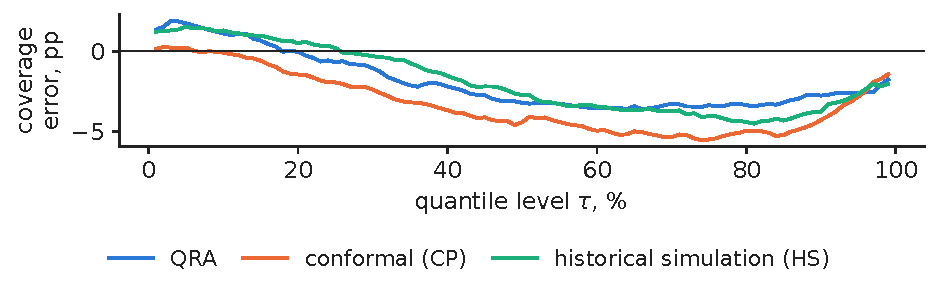
\includegraphics[width=\textwidth,height=0.457\textheight,keepaspectratio]{charts/en/prob_rel.pdf}\end{center}\vspace{-3mm}
\chartsource{Source: energy-charts.info (Fraunhofer ISE); OPCOM prices; ENTSO-E load, wind and solar (Transelectrica data for Romania). Data: test year 2025-11-01 to 2026-10-31, 99 quantiles.}
\vspace{0.5mm}
\begin{itemize}\setlength{\itemsep}{0pt}
  \item Calibrated = $\tau$\% of prices below the $\tau$-quantile (line 0)
    \begin{itemize}\setlength{\itemsep}{0pt}
      \item Above the line on the left and below on the right = tails too narrow.
    \end{itemize}
  \item Kupiec statistic for the 90\% interval: QRA 162.9, CP 83.3, HS 154.1 (5\% critical value 3.84).
\end{itemize}
\par\vfill\manager{widen the tails before using quantiles for collateral (Lecture 4).}\par\vspace{0.5mm}
\par\vfill\noindent{\scriptsize\color{FooterGray}(Kupiec, 1995, J.\ Derivatives; Gneiting \& Raftery, 2007, JASA)}\hfill\tryit{notebook \S7}\par\vspace{0.5mm}
\end{frame}

\subsection{Cointegration: prices that move together}

\begin{frame}{Two trending prices are cointegrated when their spread keeps returning}
\footnotesize
\intuition{Each price may wander, but if a combination is stationary the gap keeps closing and the regression is not spurious.}
\begin{columns}[T,onlytextwidth]
\begin{column}{0.50\textwidth}
\[ \underbrace{P^{\text{RO}}_t=\alpha+\beta P^{\text{HU}}_t+u_t}_{\text{step 1, OLS}} \]\vspace{-2mm}\[ \underbrace{\Delta\hat u_t=\rho\,\hat u_{t-1}+\textstyle\sum_j\gamma_j\Delta\hat u_{t-j}+\eta_t}_{\text{step 2, unit root in } \hat u} \]{\footnotesize\begin{itemize}\setlength{\itemsep}{0pt}
  \item \textbf{\txtwhere}
    \begin{itemize}\setlength{\itemsep}{0pt}
      \item Engle--Granger, $H_0$ no cointegration ($\rho=0$), MacKinnon critical values
      \item Johansen, trace test on the rank $r$ of a vector error-correction model.
    \end{itemize}
\end{itemize}\par}
\end{column}
\begin{column}{0.47\textwidth}
\begin{itemize}\setlength{\itemsep}{1pt}
  \item \textbf{Romania vs Hungary}, daily, since 1 Jan 2022
    \begin{itemize}\setlength{\itemsep}{0pt}
      \item $\hat\beta$ = 0.963; Engle--Granger statistic \ensuremath{-}10.58 (5\% critical value \ensuremath{-}3.34): cointegrated
      \item A shock to the spread halves in 0.8 days
    \end{itemize}
  \item \textbf{Johansen trace test}
    \begin{itemize}\setlength{\itemsep}{0pt}
      \item $r=0$: 139.7 vs 15.49; $r\le1$: 6.21 vs 3.84
      \item Rank 2, the levels are nearly stationary since 2022 (augmented Dickey--Fuller (ADF) $p$ = 0.064)
    \end{itemize}
\end{itemize}
\end{column}
\end{columns}
\par\vfill\manager{a RO--HU spread trade closes within days, not months.}\par\vspace{0.5mm}
\par\vfill\noindent{\scriptsize\color{FooterGray}(Engle \& Granger, 1987; Johansen, 1991; MacKinnon, 1996)}\hfill\tryit{notebook \S8}\par\vspace{0.5mm}
\end{frame}

\begin{frame}{Romania and Hungary: coupled markets, a spread that keeps closing}
\small
\begin{center}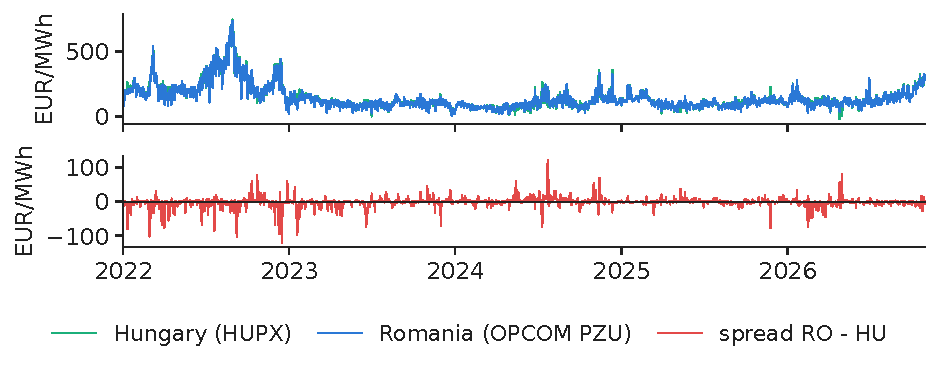
\includegraphics[width=\textwidth,height=0.437\textheight,keepaspectratio]{charts/en/coint_daily.pdf}\end{center}\vspace{-3mm}
\chartsource{Source: energy-charts.info (Fraunhofer ISE); prices of OPCOM (RO), HUPX (HU) and EPEX SPOT (DE-LU), via ENTSO-E. Data: daily base prices, 2022-01-01 to 2026-10-31.}
\vspace{0.5mm}
\begin{itemize}\setlength{\itemsep}{0pt}
  \item Spread RO $-$ HU: mean \ensuremath{-}2.07, standard deviation 15.08 EUR/MWh
    \begin{itemize}\setlength{\itemsep}{0pt}
      \item Romania vs Germany--Luxembourg: 21.06 and 37.79.
    \end{itemize}
  \item In the test year RO and HU prices were identical in 10.1\% of the hours
    \begin{itemize}\setlength{\itemsep}{0pt}
      \item The rest reflects congested borders.
    \end{itemize}
\end{itemize}
\par\vfill\manager{use the Hungarian price as a regressor or a check on your Romanian forecast.}\par\vspace{0.5mm}
\par\vfill\noindent{\scriptsize\color{FooterGray}(Engle \& Granger, 1987, Econometrica)}\hfill\tryit{notebook \S8}\par\vspace{0.5mm}
\end{frame}

\begin{frame}{Power, gas and hydro: an error-correction model on monthly data}
\footnotesize
\intuition{If price and gas are cointegrated, the price is pulled back to its gas-implied level each month, and hydro shifts it in between.}
\begin{columns}[T,onlytextwidth]
\begin{column}{0.53\textwidth}
\[ \Delta P_t=c+\underbrace{\alpha\,(P_{t-1}-a-\beta\,\text{TTF}_{t-1})}_{\text{error correction}}+\gamma\,\Delta\text{TTF}_t+\delta\,H_t+\varepsilon_t \]{\footnotesize\begin{itemize}\setlength{\itemsep}{0pt}
  \item \textbf{\txtwhere}
    \begin{itemize}\setlength{\itemsep}{0pt}
      \item $P_t$ = monthly mean price of Romania
      \item TTF in EUR/MWh
      \item $H_t$ = hydro output minus its calendar-month mean (TWh), stationary
      \item $\alpha<0$ = speed of return.
    \end{itemize}
\end{itemize}\par}
\end{column}
\begin{column}{0.44\textwidth}
\begin{itemize}\setlength{\itemsep}{1pt}
  \item \textbf{On our data}, 2015-01 -- 2026-10
    \begin{itemize}\setlength{\itemsep}{0pt}
      \item Engle--Granger \ensuremath{-}5.64 (5\% critical value \ensuremath{-}3.38); Johansen rank 1
      \item $\hat\beta$ = 1.95, as if a gas plant of about 51\% efficiency set the price
    \end{itemize}
  \item \textbf{Error-correction model (ECM)}
    \begin{itemize}\setlength{\itemsep}{0pt}
      \item $\hat\alpha$ = \ensuremath{-}0.452, half-life 1.2 months
      \item $\hat\delta$ = \ensuremath{-}12.80 EUR/MWh per TWh of extra hydro ($t$ = \ensuremath{-}3.10)
    \end{itemize}
\end{itemize}
\end{column}
\end{columns}
\par\vfill\manager{a hydro producer in a dry month can expect prices above the gas-implied level for one or two months.}\par\vspace{0.5mm}
\par\vfill\noindent{\scriptsize\color{FooterGray}(Engle \& Granger, 1987; Johansen, 1991, Econometrica)}\hfill\tryit{notebook \S8}\par\vspace{0.5mm}
\end{frame}

\begin{frame}{Power, gas and hydro: the Lecture 1 regression is not spurious}
\small
\begin{center}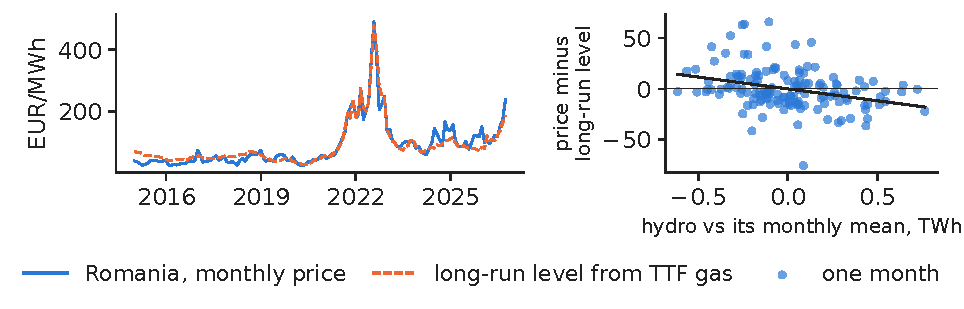
\includegraphics[width=\textwidth,height=0.527\textheight,keepaspectratio]{charts/en/coint_monthly.pdf}\end{center}\vspace{-3mm}
\chartsource{Source: energy-charts.info (OPCOM prices; ENTSO-E hydro generation, Transelectrica data); World Bank Pink Sheet (TTF). Data: monthly, 2015-01 to 2026-10.}
\vspace{0.5mm}
\begin{itemize}\setlength{\itemsep}{0pt}
  \item Left, the monthly price follows its gas-implied level
    \begin{itemize}\setlength{\itemsep}{0pt}
      \item Right, months with more hydro than usual sit below it.
    \end{itemize}
\end{itemize}
\par\vfill\manager{read a dry hydro year as a price premium over gas, not as a new price level.}\par\vspace{0.5mm}
\par\vfill\noindent{\scriptsize\color{FooterGray}(Lecture 1, hydro case; own estimation)}\hfill\tryit{notebook \S8}\par\vspace{0.5mm}
\end{frame}


\section{Case studies on recent Romanian data}

\subsection{(a) A year of forecasts}

\begin{frame}{Case study (a): a year of forecasts, month by month}
\small
\begin{center}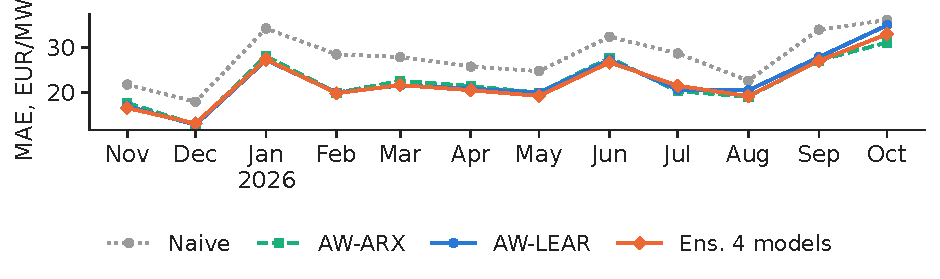
\includegraphics[width=\textwidth,height=0.500\textheight,keepaspectratio]{charts/en/monthly_mae.pdf}\end{center}\vspace{-3mm}
\chartsource{Source: energy-charts.info (Fraunhofer ISE); OPCOM prices; ENTSO-E generation and flows (Transelectrica data for Romania); Yahoo Finance (SparkChange EUA ETC). Data: test year 2025-11-01 to 2026-10-31.}
\vspace{0.5mm}
\begin{itemize}\setlength{\itemsep}{0pt}
  \item AW-LEAR beats naive in 12 of 12 months
    \begin{itemize}\setlength{\itemsep}{0pt}
      \item MAE from 12.84 (Dec 2025) to 34.88 EUR/MWh (Oct 2026).
    \end{itemize}
\end{itemize}
\par\vfill\manager{report accuracy by month, since a good annual MAE can hide a bad autumn.}\par\vspace{0.5mm}
\par\vfill\noindent{\scriptsize\color{FooterGray}(own computation, test year 1 Nov 2025 -- 31 Oct 2026)}\hfill\tryit{notebook \S9}\par\vspace{0.5mm}
\end{frame}

\subsection{(b) A stress week}

\begin{frame}{Case study (b): the stress week of 19 Oct 2026}
\small
\begin{center}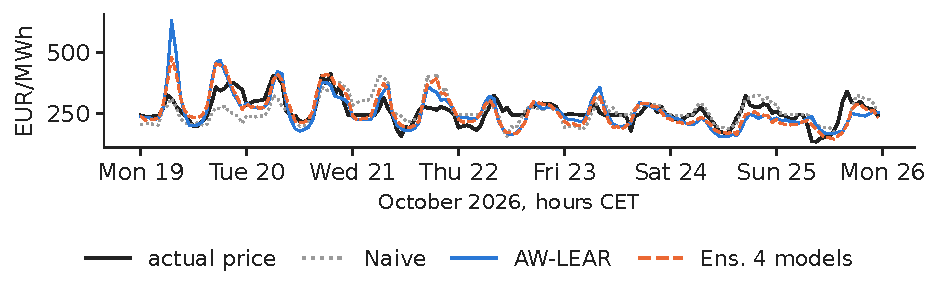
\includegraphics[width=\textwidth,height=0.500\textheight,keepaspectratio]{charts/en/stress_week.pdf}\end{center}\vspace{-3mm}
\chartsource{Source: energy-charts.info (Fraunhofer ISE); OPCOM prices; ENTSO-E generation and flows (Transelectrica data for Romania); Yahoo Finance (SparkChange EUA ETC). Data: week 2026-10-19 to 2026-10-25, hourly.}
\vspace{0.5mm}
\begin{itemize}\setlength{\itemsep}{0pt}
  \item Mean 258.59, peak 412.35 EUR/MWh
    \begin{itemize}\setlength{\itemsep}{0pt}
      \item MAE naive 40.19, AW-LEAR 36.54, GBM 34.35, ensemble 34.95.
    \end{itemize}
\end{itemize}
\par\vfill\manager{every model lags a jump in level by a day, so hedge the evening hours.}\par\vspace{0.5mm}
\par\vfill\noindent{\scriptsize\color{FooterGray}(own computation; OPCOM)}\hfill\tryit{notebook \S9}\par\vspace{0.5mm}
\end{frame}

\subsection{(c) The 15-minute market time unit}

\begin{frame}{Case study (c): forecasting 96 quarter-hours since 1 October 2025}
\small
\begin{center}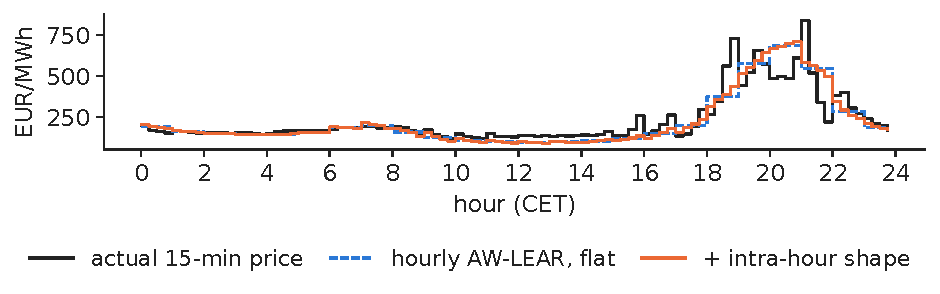
\includegraphics[width=\textwidth,height=0.387\textheight,keepaspectratio]{charts/en/mtu15.pdf}\end{center}\vspace{-3mm}
\chartsource{Source: energy-charts.info (Fraunhofer ISE); OPCOM 15-minute day-ahead prices for Romania, via ENTSO-E. Data: 2026-07-01, 96 quarter-hours (CET).}
\vspace{0.5mm}
\begin{itemize}\setlength{\itemsep}{0pt}
  \item The market time unit (MTU) is 15 minutes
    \begin{itemize}\setlength{\itemsep}{0pt}
      \item Forecast = hourly AW-LEAR + the mean intra-hour shape of the 28 previous days.
    \end{itemize}
  \item 363 test days without DST, quarter-hour MAE 26.02 flat vs 24.53 EUR/MWh shaped.
\end{itemize}
\par\vfill\manager{a battery bids per quarter-hour
    \begin{itemize}\setlength{\itemsep}{0pt}
      \item Give it the intra-hour shape, not a flat hour.
    \end{itemize}}\par\vspace{0.5mm}
\par\vfill\noindent{\scriptsize\color{FooterGray}(own computation; OPCOM; SDAC 15-minute go-live, 1 Oct 2025)}\hfill\tryit{notebook \S9}\par\vspace{0.5mm}
\end{frame}

\subsection{(d) From forecast to money}

\begin{frame}{Case study (d): what a better forecast is worth}
\small
\begin{center}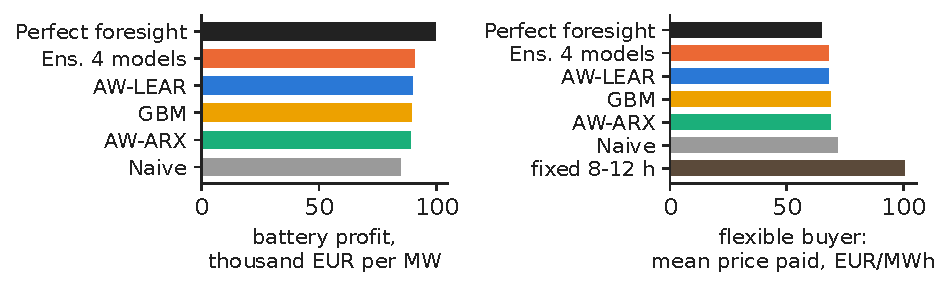
\includegraphics[width=\textwidth,height=0.410\textheight,keepaspectratio]{charts/en/battery.pdf}\end{center}\vspace{-3mm}
\chartsource{Source: energy-charts.info (Fraunhofer ISE); OPCOM prices; ENTSO-E generation and flows (Transelectrica data for Romania); Yahoo Finance (SparkChange EUA ETC). Data: test year 2025-11-01 to 2026-10-31; 1 MW / 2 MWh, round-trip efficiency 90\%.}
\vspace{0.5mm}
\begin{itemize}\setlength{\itemsep}{0pt}
  \item Battery 1 MW / 2 MWh, one daily cycle set on the forecast, 363 days without DST, 90\,738 EUR per MW with the ensemble (91.0\% of perfect foresight), 84\,623 with naive.
  \item Flexible 4-hour process of a supplier, 67.87 EUR/MWh with AW-LEAR vs 100.59 for a fixed 8--12 h CET block.
\end{itemize}
\par\vfill\manager{translate rMAE into EUR before paying for a forecast.}\par\vspace{0.5mm}
\par\vfill\noindent{\scriptsize\color{FooterGray}(own computation; round-trip efficiency 90\% assumed)}\hfill\tryit{notebook \S9}\par\vspace{0.5mm}
\end{frame}

\begin{frame}{A forecasting desk checklist, and our leakage self-check}
\footnotesize
\begin{columns}[T,onlytextwidth]
\begin{column}{0.52\textwidth}
\begin{itemize}\setlength{\itemsep}{1pt}
  \item \textbf{Before you trust a backtest}
    \begin{itemize}\setlength{\itemsep}{0pt}
      \item Every input public before 12:00 CET on $d-1$
      \item Scalers, transforms, $\lambda$ and thresholds fitted in the window only
      \item Chronological validation; the test year touched once
    \end{itemize}
  \item \textbf{Then report}
    \begin{itemize}\setlength{\itemsep}{0pt}
      \item MAE and rMAE against naive, DM $p$-values, coverage of the intervals
      \item Results by month and by hour, not only one annual number
    \end{itemize}
\end{itemize}
\end{column}
\begin{column}{0.45\textwidth}
\begin{itemize}\setlength{\itemsep}{1pt}
  \item \textbf{Our self-check} (analysis script, section 7)
    \begin{itemize}\setlength{\itemsep}{0pt}
      \item 9\,364 timestamp checks, each input at least 12 h before the cut-off
      \item 17 forecast series recomputed on 14 days, GBM and MLP on the first day of all 12 refits
      \item Later data deleted or replaced by nonsense; forecasts identical up to rounding
      \item Status: passed
    \end{itemize}
\end{itemize}
\end{column}
\end{columns}
\par\vfill\manager{make the leakage check part of every model review, as Assignment 1 does.}\par\vspace{0.5mm}
\par\vfill\noindent{\scriptsize\color{FooterGray}(Assignment 1; Lago et al., 2021, APEN)}\hfill\tryit{notebook \S10}\par\vspace{0.5mm}
\end{frame}

\section*{Wrap-up}

\begin{frame}{Quiz 1: the naive rule on a Monday}
\small
\begin{itemize}
  \item It is Sunday, 11:30 CET
    \begin{itemize}\setlength{\itemsep}{0pt}
      \item You must forecast Monday, hour 19:00, with the naive benchmark
      \item Which price do you use?
    \end{itemize}
\end{itemize}
\vspace{2mm}
\begin{exampleblock}{Answer}
\begin{itemize}
  \item The price of the previous Monday at 19:00 ($d-7$)
    \begin{itemize}\setlength{\itemsep}{0pt}
      \item On our test year this beats Sunday's price on Mon, Sat and Sun (MAE 29.87 vs 33.48 EUR/MWh).
    \end{itemize}
\end{itemize}
\end{exampleblock}
\end{frame}

\begin{frame}{Quiz 2: a suspicious backtest}
\small
\begin{itemize}
  \item A vendor reports rMAE 0.55 for Romania and uses the realised load of day $d-1$ as a regressor
    \begin{itemize}\setlength{\itemsep}{0pt}
      \item Do you buy?
    \end{itemize}
\end{itemize}
\vspace{2mm}
\begin{exampleblock}{Answer}
\begin{itemize}
  \item No: at 12:00 on $d-1$ that day is not yet metered, so the backtest leaks information
    \begin{itemize}\setlength{\itemsep}{0pt}
      \item Ask for a rerun with data up to $d-2$ (or published day-ahead forecasts)
      \item Our honest best is rMAE 0.795.
    \end{itemize}
\end{itemize}
\end{exampleblock}
\end{frame}

\begin{frame}{Quiz 3: reading a DM test}
\small
\begin{itemize}
  \item AW-ARX or AW-LEAR? The DM test gives $p$ = 0.797
    \begin{itemize}\setlength{\itemsep}{0pt}
      \item Which model goes into production?
    \end{itemize}
\end{itemize}
\vspace{2mm}
\begin{exampleblock}{Answer}
\begin{itemize}
  \item Neither wins significantly
    \begin{itemize}\setlength{\itemsep}{0pt}
      \item Take the simpler one, or better their average, which is part of the best ensemble (rMAE 0.795).
    \end{itemize}
\end{itemize}
\end{exampleblock}
\end{frame}

\begin{frame}{Quiz 4: an error measure for the board}
\small
\begin{itemize}
  \item Your report shows MAPE 5\,778\% for the Romanian price forecast
    \begin{itemize}\setlength{\itemsep}{0pt}
      \item The board is alarmed
      \item What do you say?
    \end{itemize}
\end{itemize}
\vspace{2mm}
\begin{exampleblock}{Answer}
\begin{itemize}
  \item MAPE divides by prices near zero ($387$ hours below 5 EUR/MWh produce 99.5\% of it)
    \begin{itemize}\setlength{\itemsep}{0pt}
      \item Report MAE 22.53 EUR/MWh and rMAE 0.810 instead.
    \end{itemize}
\end{itemize}
\end{exampleblock}
\end{frame}

\begin{frame}{Quiz 5: cointegration in practice}
\small
\begin{itemize}
  \item The RO--HU spread is cointegrated with a half-life of 0.8 days
    \begin{itemize}\setlength{\itemsep}{0pt}
      \item Today Romania is 40 EUR/MWh above Hungary
      \item What do you expect?
    \end{itemize}
\end{itemize}
\vspace{2mm}
\begin{exampleblock}{Answer}
\begin{itemize}
  \item The gap should shrink by about half within a day, unless the border stays congested
    \begin{itemize}\setlength{\itemsep}{0pt}
      \item It is a signal for cross-border trading, not a guarantee.
    \end{itemize}
\end{itemize}
\end{exampleblock}
\end{frame}

\begin{frame}{Wrap-up}
\small
\vspace{-2mm}\begin{multicols}{2}\scriptsize\tableofcontents\end{multicols}
\begin{itemize}\setlength{\itemsep}{1pt}
  \item Honest setup first: information at 12:00 CET on $d-1$, rolling windows, naive benchmark, DM tests.
  \item On the test year the best model, an ensemble of 4, cuts the naive error by 20.5\%
    \begin{itemize}\setlength{\itemsep}{0pt}
      \item Next: volatility (Lecture 3).
    \end{itemize}
\end{itemize}
\end{frame}

\begin{frame}{Research from our group on forecasting Romanian power}
\footnotesize
\begin{itemize}\setlength{\itemsep}{1pt}
  \item \textbf{Benchmarking load forecasts}: classical seasonal models against neural networks on Romania's national consumption
    \begin{itemize}\setlength{\itemsep}{0pt}
      \item In the paper a neural network has a clearly lower error than the seasonal autoregressive benchmark (Proșcanu, Proșcanu, Pele \& Costea, 2025, RJEF) --- case study C2.
    \end{itemize}
  \item \textbf{Four generations of price models}: a comparative evaluation of four generations of forecasting methods for energy prices, a reference for choosing a model family (Andrei, Velev, Toma, Pele \& Lessmann, 2024, arXiv 2411.03372).
  \item \textbf{Explaining price forecasts across horizons}: which drivers matter at which horizon and in which price regime, for Romanian hourly prices (Andrei, Pele \& Cramer, 2026, PICBE).
  \item \textbf{Early warning of price spikes}: an explainable artificial intelligence (AI) system in which the previous price and the residual load drive the spikes (Andrei, Pele, Cramer, Amza \& Diaconu, 2026, PICBE) --- preview of Lecture 7.
\end{itemize}
\par\vspace{0.5mm}{\scriptsize \begin{itemize}\setlength{\itemsep}{0pt}
  \item Findings as stated in the papers; numbers on the other slides come from our own data.
\end{itemize}}
\par\vfill\noindent{\scriptsize\color{FooterGray}(Bucharest University of Economic Studies; Romanian Academy, Institute for Economic Forecasting)}\par\vspace{0.5mm}
\end{frame}

\begin{frame}{Want to learn more?}
\small
\begin{columns}[T,onlytextwidth]
\begin{column}{0.52\textwidth}
\begin{itemize}\setlength{\itemsep}{1pt}
  \item \textbf{R.\ Weron, IIF Distinguished Lectures on electricity price forecasting} (2025): slides \href{https://p.wz.pwr.edu.pl/~weron.rafal/assets/PDF/Weron25_IIF_1.pdf}{part I}, \href{https://p.wz.pwr.edu.pl/~weron.rafal/assets/PDF/Weron25_IIF_2.pdf}{part II}, \href{https://github.com/lipiecki/energy-analytics-2025}{notebooks}.
  \item \textbf{epftoolbox}, LEAR and DNN with the open benchmark of Lago et al.\ (2021): \href{https://github.com/jeslago/epftoolbox}{github.com/jeslago/epftoolbox}.
  \item \textbf{Forecasting -- Principles and Practice}, 3rd ed., \href{https://otexts.com/fpp3/}{otexts.com/fpp3}.
\end{itemize}
\end{column}
\begin{column}{0.45\textwidth}
\begin{itemize}\setlength{\itemsep}{1pt}
  \item \textbf{This course}: code, data, notebooks --- \href{https://github.com/danpele/EMQA}{github.com/danpele/EMQA}.
  \item \textbf{Assignment 1} applies ARX, LEAR, DM and the HS/CP intervals to your own test window.
  \item \textbf{Experiment yourself}: the notebook reproduces every chart and number of this lecture --- \href{\emqarepo/\emqanb}{notebooks/}.
\end{itemize}
\end{column}
\end{columns}
\end{frame}

\begin{frame}{References (1/3)}
\scriptsize
\begin{itemize}\setlength{\itemsep}{1pt}\scriptsize
\item Andrei, A.-V., Pele, D.-T.\ \& Cramer, A.-A.\ (2026). Multi-horizon explainability in energy price forecasting: Disentangling market dynamics and renewable intermittency in Romania's liberalized electricity market. \textit{Proceedings of the International Conference on Business Excellence}, 20(1), 104--117. \href{https://doi.org/10.2478/picbe-2026-0014}{doi:10.2478/picbe-2026-0014}
\item Andrei, A.-V., Pele, D.-T., Cramer, A.-A., Amza, A.\ \& Diaconu, D.\ (2026). Explainable AI-based early warning system for electricity price spikes: Evidence from the Romanian market. \textit{Proceedings of the International Conference on Business Excellence}, 20(1), 4820--4836. \href{https://doi.org/10.2478/picbe-2026-0352}{doi:10.2478/picbe-2026-0352}
\item Andrei, A.-V., Velev, G., Toma, F.-M., Pele, D.\,T.\ \& Lessmann, S.\ (2024). Energy price modelling: A comparative evaluation of four generations of forecasting methods. arXiv:2411.03372.
\item Bates, J.\,M.\ \& Granger, C.\,W.\,J.\ (1969). The combination of forecasts. \textit{Operational Research Quarterly}, 20(4), 451--468.
\item Diebold, F.\,X.\ \& Mariano, R.\,S.\ (1995). Comparing predictive accuracy. \textit{Journal of Business \& Economic Statistics}, 13(3), 253--263.
\item Engle, R.\,F.\ \& Granger, C.\,W.\,J.\ (1987). Co-integration and error correction: Representation, estimation, and testing. \textit{Econometrica}, 55(2), 251--276. \href{https://doi.org/10.2307/1913236}{doi:10.2307/1913236}
\item Friedman, J.\,H.\ (2001). Greedy function approximation: A gradient boosting machine. \textit{Annals of Statistics}, 29(5), 1189--1232. \href{https://doi.org/10.1214/aos/1013203451}{doi:10.1214/aos/1013203451}
\item Gneiting, T.\ \& Raftery, A.\,E.\ (2007). Strictly proper scoring rules, prediction, and estimation. \textit{Journal of the American Statistical Association}, 102(477), 359--378. \href{https://doi.org/10.1198/016214506000001437}{doi:10.1198/016214506000001437}
\item Hubicka, K., Marcjasz, G.\ \& Weron, R.\ (2019). A note on averaging day-ahead electricity price forecasts across calibration windows. \textit{IEEE Transactions on Sustainable Energy}, 10(1), 321--323.
\end{itemize}
\end{frame}

\begin{frame}{References (2/3)}
\scriptsize
\begin{itemize}\setlength{\itemsep}{1pt}\scriptsize
\item Hyndman, R.\,J.\ \& Koehler, A.\,B.\ (2006). Another look at measures of forecast accuracy. \textit{International Journal of Forecasting}, 22(4), 679--688. \href{https://doi.org/10.1016/j.ijforecast.2006.03.001}{doi:10.1016/j.ijforecast.2006.03.001}
\item Johansen, S.\ (1991). Estimation and hypothesis testing of cointegration vectors in Gaussian vector autoregressive models. \textit{Econometrica}, 59(6), 1551--1580. \href{https://doi.org/10.2307/2938278}{doi:10.2307/2938278}
\item Koenker, R.\ \& Bassett, G.\ (1978). Regression quantiles. \textit{Econometrica}, 46(1), 33--50. \href{https://doi.org/10.2307/1913643}{doi:10.2307/1913643}
\item Kupiec, P.\,H.\ (1995). Techniques for verifying the accuracy of risk measurement models. \textit{Journal of Derivatives}, 3(2), 73--84.
\item Lago, J., Marcjasz, G., De Schutter, B.\ \& Weron, R.\ (2021). Forecasting day-ahead electricity prices: A review of state-of-the-art algorithms, best practices and an open-access benchmark. \textit{Applied Energy}, 293, 116983. \href{https://doi.org/10.1016/j.apenergy.2021.116983}{doi:10.1016/j.apenergy.2021.116983}
\item NEMO Committee (2025). 15-Minute MTU in SDAC was implemented. SDAC press release, 1 October 2025. \href{https://nemo-committee.eu/assets/files/15-minute-mtu-in-sdac-was-implemented.pdf}{nemo-committee.eu}
\item NEMO Committee (2026). Single Day-Ahead Coupling (SDAC) and the EUPHEMIA algorithm. \href{https://www.nemo-committee.eu/sdac}{nemo-committee.eu/sdac}
\item MacKinnon, J.\,G.\ (1996). Numerical distribution functions for unit root and cointegration tests. \textit{Journal of Applied Econometrics}, 11(6), 601--618.
\item Marcjasz, G., Serafin, T.\ \& Weron, R.\ (2018). Selection of calibration windows for day-ahead electricity price forecasting. \textit{Energies}, 11(9), 2364.
\end{itemize}
\end{frame}

\begin{frame}{References (3/3)}
\scriptsize
\begin{itemize}\setlength{\itemsep}{1pt}\scriptsize
\item Nogales, F.\,J., Contreras, J., Conejo, A.\,J.\ \& Espínola, R.\ (2002). Forecasting next-day electricity prices by time series models. \textit{IEEE Transactions on Power Systems}, 17(2), 342--348. \href{https://doi.org/10.1109/TPWRS.2002.1007902}{doi:10.1109/TPWRS.2002.1007902}
\item Nowotarski, J.\ \& Weron, R.\ (2015). Computing electricity spot price prediction intervals using quantile regression and forecast averaging. \textit{Computational Statistics}, 30(3), 791--803. \href{https://doi.org/10.1007/s00180-014-0523-0}{doi:10.1007/s00180-014-0523-0}
\item Nowotarski, J.\ \& Weron, R.\ (2018). Recent advances in electricity price forecasting: A review of probabilistic forecasting. \textit{Renewable and Sustainable Energy Reviews}, 81, 1548--1568. \href{https://doi.org/10.1016/j.rser.2017.05.234}{doi:10.1016/j.rser.2017.05.234}
\item Proșcanu, C.\,A., Proșcanu, M.\,E., Pele, D.\,T.\ \& Costea, A.\ (2025). Watt's next? Benchmarking time series models on Romania's national electricity consumption. \textit{Romanian Journal of Economic Forecasting}, 28(3), 146--163.
\item Tibshirani, R.\ (1996). Regression shrinkage and selection via the lasso. \textit{Journal of the Royal Statistical Society B}, 58(1), 267--288. \href{https://doi.org/10.1111/j.2517-6161.1996.tb02080.x}{doi:10.1111/j.2517-6161.1996.tb02080.x}
\item Uniejewski, B., Nowotarski, J.\ \& Weron, R.\ (2016). Automated variable selection and shrinkage for day-ahead electricity price forecasting. \textit{Energies}, 9(8), 621. \href{https://doi.org/10.3390/en9080621}{doi:10.3390/en9080621}
\item Uniejewski, B., Weron, R.\ \& Ziel, F.\ (2018). Variance stabilizing transformations for electricity spot price forecasting. \textit{IEEE Transactions on Power Systems}, 33(2), 2219--2229. \href{https://doi.org/10.1109/TPWRS.2017.2734563}{doi:10.1109/TPWRS.2017.2734563}
\item Weron, R.\ (2014). Electricity price forecasting: A review of the state-of-the-art with a look into the future. \textit{International Journal of Forecasting}, 30(4), 1030--1081. \href{https://doi.org/10.1016/j.ijforecast.2014.08.008}{doi:10.1016/j.ijforecast.2014.08.008}
\item Ziel, F.\ \& Weron, R.\ (2018). Day-ahead electricity price forecasting with high-dimensional structures: Univariate vs.\ multivariate modeling frameworks. \textit{Energy Economics}, 70, 396--420. \href{https://doi.org/10.1016/j.eneco.2017.12.016}{doi:10.1016/j.eneco.2017.12.016}
\end{itemize}
\end{frame}

\appendix

\section*{Appendix}

\begin{frame}{Appendix A: LEAR in full}
\small
\begin{columns}[T,onlytextwidth]
\begin{column}{0.55\textwidth}
\[ \text{AIC}(\lambda)=n\ln\frac{\text{RSS}(\lambda)}{n}+2\,\mathrm{df}(\lambda) \]\begin{itemize}\setlength{\itemsep}{1pt}
  \item Residual sum of squares (RSS)
    \begin{itemize}\setlength{\itemsep}{0pt}
      \item The degrees of freedom df($\lambda$) = number of non-zero coefficients
      \item Path by least angle regression (LARS), in scikit-learn.
    \end{itemize}
  \item Price block: $m$, $s$ = median and $1.4826\cdot$MAD of the prices of rows $d-T-7,\dots,d-1$, pooled over 24 hours.
  \item Load and wind + solar: own asinh transform from rows up to $d-2$
    \begin{itemize}\setlength{\itemsep}{0pt}
      \item Then every column z-scored on the calibration rows.
    \end{itemize}
\end{itemize}
\end{column}
\begin{column}{0.42\textwidth}
{\footnotesize\renewcommand{\arraystretch}{1.15}\setlength{\tabcolsep}{4pt}
\begin{tabular}{@{}lr@{}}\toprule
Block & Columns \\ \midrule
prices $d-1$, all 24 hours & 24 \\
prices $d-2$, $d-3$, $d-7$ & 72 \\
load $d-2$, $d-3$, $d-7$ & 72 \\
wind + solar $d-2$, $d-3$, $d-7$ & 72 \\
day of week & 7 \\
\textbf{total} & \textbf{247} \\
\bottomrule\end{tabular}}
\end{column}
\end{columns}
\par\vfill\noindent{\scriptsize\color{FooterGray}(Uniejewski, Nowotarski \& Weron, 2016, Energies; Lago et al., 2021, APEN)}\par\vspace{0.5mm}
\end{frame}

\begin{frame}{Appendix B: MAE by quarter of the test year}
\small
\begin{center}{\footnotesize\renewcommand{\arraystretch}{1.15}\setlength{\tabcolsep}{4pt}
\begin{tabular}{@{}lrrrrr@{}}\toprule
Model & 2025 Q4 & 2026 Q1 & 2026 Q2 & 2026 Q3 & 2026 Q4 \\ \midrule
naive & \cellcolor{Crimson!55}19.80 & \cellcolor{Crimson!55}30.19 & \cellcolor{Crimson!55}27.55 & \cellcolor{Crimson!55}28.32 & \cellcolor{Forest!3}36.05 \\
AW-ARX & \cellcolor{Forest!46}15.24 & \cellcolor{Forest!45}23.62 & \cellcolor{Forest!37}22.97 & \cellcolor{Forest!55}22.09 & \cellcolor{Forest!55}31.05 \\
AW-LEAR & \cellcolor{Forest!54}14.86 & \cellcolor{Forest!55}22.99 & \cellcolor{Forest!44}22.64 & \cellcolor{Forest!41}22.91 & \cellcolor{Forest!15}34.88 \\
GBM & \cellcolor{Forest!23}16.25 & \cellcolor{Forest!29}24.71 & \cellcolor{Forest!37}22.98 & \cellcolor{Forest!4}24.97 & \cellcolor{Crimson!16}37.88 \\
MLP & \cellcolor{Forest!1}17.27 & \cellcolor{Forest!17}25.49 & \cellcolor{Crimson!1}24.89 & \cellcolor{Crimson!19}26.30 & \cellcolor{Crimson!55}41.58 \\
ensemble of 4 & \cellcolor{Forest!55}14.82 & \cellcolor{Forest!55}23.02 & \cellcolor{Forest!55}22.09 & \cellcolor{Forest!48}22.50 & \cellcolor{Forest!36}32.91 \\
\bottomrule\end{tabular}}\end{center}
\par\vspace{0.5mm}{\scriptsize \begin{itemize}\setlength{\itemsep}{0pt}
  \item Days per quarter: 61, 90, 91, 92, 31 (the test year starts on 1 Nov 2025).
  \item Green = best in that quarter, red = worst.
\end{itemize}}
\par\vfill\noindent{\scriptsize\color{FooterGray}(Weron, 2014, IJF; Lago, Marcjasz, De Schutter \& Weron, 2021, APEN)}\par\vspace{0.5mm}
\end{frame}

\begin{frame}{Appendix C: probabilistic scores and the Kupiec test}
\footnotesize
\begin{columns}[T,onlytextwidth]
\begin{column}{0.50\textwidth}
\[ \text{LR}_{\text{UC}}=-2\ln\frac{(1-p_0)^{n-x}p_0^{\,x}}{(1-\hat p)^{n-x}\hat p^{\,x}}\sim\chi^2_1,\quad \hat p=\frac xn \]\begin{itemize}\setlength{\itemsep}{1pt}
  \item Likelihood ratio (LR) for unconditional coverage (UC)
    \begin{itemize}\setlength{\itemsep}{0pt}
      \item $x$ = hours outside the 90\% interval out of $n$ = 8\,760
      \item $p_0=0.10$.
    \end{itemize}
  \item Hours of the same day are not independent, so the test is indicative
    \begin{itemize}\setlength{\itemsep}{0pt}
      \item A test on the daily miss share with Newey--West variance gives $p$ = $<$0.001 for QRA.
    \end{itemize}
  \item Pinball score averaged over 99 quantiles
    \begin{itemize}\setlength{\itemsep}{0pt}
      \item The continuous ranked probability score $\approx 2\times$ this score.
    \end{itemize}
\end{itemize}
\end{column}
\begin{column}{0.47\textwidth}
{\footnotesize\renewcommand{\arraystretch}{1.2}\setlength{\tabcolsep}{4pt}
\begin{tabular}{@{}lrrrr@{}}\toprule
Method & Pinball & Cov.\ 50\% & Cov.\ 90\% & Kupiec \\ \midrule
QRA & 8.33 & 47.3 & 85.7 & 162.9 \\
CP & 8.47 & 46.5 & 87.0 & 83.3 \\
HS & 8.41 & 45.8 & 85.8 & 154.1 \\
\bottomrule\end{tabular}}
\end{column}
\end{columns}
\par\vfill\noindent{\scriptsize\color{FooterGray}(Kupiec, 1995; Gneiting \& Raftery, 2007, JASA)}\par\vspace{0.5mm}
\end{frame}

\begin{frame}{Appendix D: unit-root and cointegration tests in full}
\small
\begin{center}{\footnotesize\renewcommand{\arraystretch}{1.1}\setlength{\tabcolsep}{4pt}
\begin{tabular}{@{}llrr@{}}\toprule
Series / pair & Test & Statistic & $p$ / crit.\ 5\% \\ \midrule
RO, HU, DE-LU daily levels & ADF $p$ & -- & 0.064, 0.052, 0.015 \\
RO--HU & Engle--Granger & \ensuremath{-}10.58 & \ensuremath{-}3.34 \\
RO--HU & Johansen $r=0$ / $r\le1$ & 139.7 / 6.21 & 15.49 / 3.84 \\
RO--DE-LU & Engle--Granger & \ensuremath{-}5.79 & \ensuremath{-}3.34 \\
RO price, TTF, monthly levels & ADF $p$ & -- & 0.295, 0.249 \\
hydro minus monthly mean & ADF $p$ & -- & 0.002 \\
price--TTF & Engle--Granger & \ensuremath{-}5.64 & \ensuremath{-}3.38 \\
price--TTF--hydro & Engle--Granger & \ensuremath{-}5.95 & \ensuremath{-}3.80 \\
price--TTF & Johansen $r=0$ / $r\le1$ & 21.32 / 3.74 & 15.49 / 3.84 \\
\bottomrule\end{tabular}}\end{center}
\par\vspace{0.5mm}{\scriptsize \begin{itemize}\setlength{\itemsep}{0pt}
  \item ADF with AIC lags; Johansen with a constant, 6 lagged differences (daily) or 2 (monthly).
  \item ECM with heteroskedasticity- and autocorrelation-robust standard errors (6 lags), 141 months, $R^2$ = 0.778.
\end{itemize}}
\par\vfill\noindent{\scriptsize\color{FooterGray}(Engle \& Granger, 1987; Johansen, 1991; MacKinnon, 1996)}\par\vspace{0.5mm}
\end{frame}

\end{document}
